\documentclass[10pt,xcolor={svgnames}]{beamer}
%\usefonttheme[onlymath]{serif}
%%%%% Colors
\usetheme{Dresden}%\usetheme{Madrid}
\colorlet{beamer@blendedblue}{green!55!black}
%%%%%

%%%%% Other 
\beamertemplatenavigationsymbolsempty
\addtobeamertemplate{navigation symbols}{}{%
    \usebeamerfont{footline}%
    \usebeamercolor[fg]{footline}%
    \hspace{1em}%
    \insertframenumber/\inserttotalframenumber
}
\usepackage{hyperref, url}
%\usepackage[symbol]{footmisc}

\definecolor{pine_green}{HTML}{007935}
\hypersetup{colorlinks,breaklinks,linkcolor=white,urlcolor=orange,citecolor=black}
\renewcommand\thefootnote{\textcolor{pine_green}{\arabic{footnote}}}
\setbeamercolor{alerted text}{fg=pine_green}

\renewcommand{\i}{\mathnormal{I}}

\usepackage{cancel}
\usepackage{ulem}
\usepackage{multirow}
\usepackage{mathtools}
\usepackage{makecell}
\DeclarePairedDelimiter{\abs}{\lvert}{\rvert}
\renewcommand{\epsilon}{\varepsilon}
\setbeamertemplate{itemize subitem}{\textbullet}
\setbeamertemplate{itemize subsubitem}{$\circ$}

%https://tex.stackexchange.com/questions/289542/auto-resizing-parenthesis-in-math-formulas
% \usepackage{amsmath} for testing
\newcommand*\autoop{\left(}
\newcommand*\autocp{\right)}
\newcommand*\autoob{\left[}
\newcommand*\autocb{\right]}
\AtBeginDocument {%
   \mathcode`( 32768
   \mathcode`) 32768
   \mathcode`[ 32768
   \mathcode`] 32768
   \begingroup
       \lccode`\~`(
       \lowercase{%
   \endgroup
       \let~\autoop
   }\begingroup
       \lccode`\~`)
       \lowercase{%
   \endgroup
       \let~\autocp
   }\begingroup
       \lccode`\~`[
       \lowercase{%
   \endgroup
       \let~\autoob
   }\begingroup
       \lccode`\~`]
       \lowercase{%
   \endgroup
       \let~\autocb
   }}

\delimiterfactor 1001

\makeatletter
% for amsmath "compatibility" (not sophisticated)
% \usepackage{amsmath}
\AtBeginDocument {%
          \def\resetMathstrut@{%
           \setbox\z@\hbox{\the\textfont\symoperators\char40}%
           \ht\Mathstrutbox@\ht\z@ \dp\Mathstrutbox@\dp\z@}%
}%
\makeatother
%%%%%

%%%%% Greying out/invidible Slides
%\setbeamercovered{invisible}
%\setbeamercovered{%
%  again covered={\opaqueness<1->{15}}}
  
%%%%%







%%%%% Footnotes and captions
%\usepackage[utf8]{inputenc}
\usepackage{caption}
\usepackage{comment}
\setbeamerfont{footnote}{size=\tiny}
\setbeamerfont{caption}{size=\small}
%\setbeamerfont{normal text}{size=\small}
\setbeamerfont{itemize/enumerate body}{size=\small}
\setbeamerfont{itemize/enumerate subbody}{size=\footnotesize}
%%%%%



%Information to be included in the title page:
\title[Connor Wiegand]{Intro to Economic Analysis: Microeconomics}
\subtitle{EC 201 - Day 9 Slides}
\author[EC 201]{Connor Wiegand}
\institute[]{Department of Economics - University of Oregon}
\date{25 October 2021}


\begin{document}

\frame{\titlepage}

\section*{Recap}

\begin{frame}{Logistics}
    \begin{itemize}
        \item Official homework 4 due this Saturday at 11:59pm, covering last week's material
        \item Next news assignments posted, due this Wednesday (October 27)
        \item Midterm Wednesday, November 3rd
        \begin{itemize}
            \item Read the announcement about class-designed note card
            \item Bring non-graphing, non-algebra calculator
            \item Bring \#2 Pencil (yes it has to be \#2)
        \end{itemize}
    \end{itemize}
\end{frame}

\begin{frame}{Willingness to Accept}
    \begin{itemize}[<+->]
        \item Motivating and defining producer surplus looks a lot like consumer surplus
        \item Producers have a ``willingness to accept": the minimum price that a producer will take in order to sell a product
        \item A producer's \underline{\textbf{Total Willingness to Accept}} (TWTA) is the minimum amount a producer will take in order to sell a specific quantity of a good
        \item A consumer's \underline{\textbf{Marginal Willingness to Accept}} (MWTA) is the  minimum amount a producer will take to sell the \underline{next}\footnote{\vspace{1mm} Again, ``last", depending on context} unit of a good
    \end{itemize}
\end{frame}


\begin{frame}{Producer Surplus Motivation}
    \begin{itemize}[<+->]
        \item Suppose it only costs Caspian \$2 to make a breakfast pita, so they are willing to accept \$2
        \item However, the market price of a breakfast pita is \$4
        \item Caspian gets a ``bonus" from selling the pita at a higher price than it's worth -- in this case, profit
        \footnote{One could conceive that a producer is endowed with some goods, and still has some minimum price they are willing to sell at. Thus, producer surplus need not always equal profit}
        \item Other sellers of breakfast pitas may be willing to accept \$1, some \$3.50, etc. 
        \item Each of them gets an individual surplus from getting a ``deal" on their pita, as long as their WTA is low enough to sell the product $(\leq \$4)$
        \item If we add these surplus values up, for everyone who sold the pita, then we get what we call the \underline{producer surplus}
    \end{itemize}
\end{frame}

\begin{frame}{Producer Surplus Definition}
    \begin{itemize}[<+->]
        \item \underline{\textit{[Individual] Producer Surplus}} is the difference between a seller's WTA and the price they actually sell for \footnote{Throughout: assuming this value is positive, i.e. assuming they sold the product}
        \item \underline{\textbf{Producer Surplus}} is the the sum of all individual producer surplus's; i.e., it is the area between the WTA reflected by the market supply curve, and the price at which the good was sold
        \item Producer surplus is our measure for the overall utility (often thought of as profit), or ``welfare", on the seller's side of the market
        \item Selling a product gives the producer happiness through money, but working to produce and parting with the product took away some happiness. Whatever is leftover is the economic well-being of producers in the market
    \end{itemize}
\end{frame}


\begin{frame}{Graphical Representation of CS \& PS}
    \begin{figure}
        \centering
        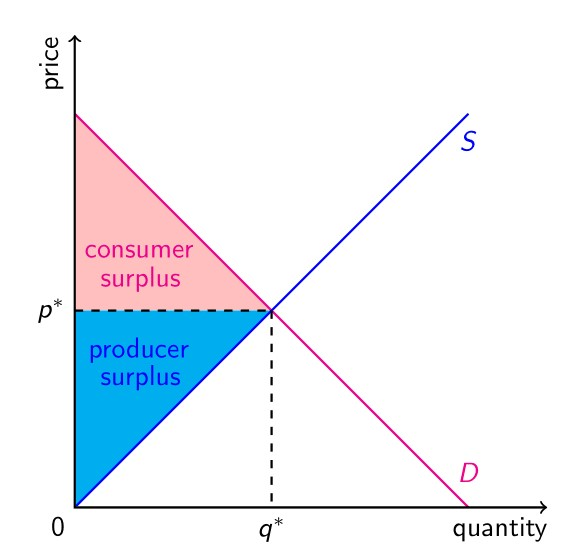
\includegraphics[width=7cm]{cs-ps simple.png}
    \end{figure}
\end{frame}


\begin{frame}{CS/PS Exercise 1}
    \begin{itemize}
        \item Recall that the area of a triangle is $\frac{1}{2}$ base times height
        \item Compute consumer, producer, and total surplus for hot dogs 
    \begin{figure}
        \centering
        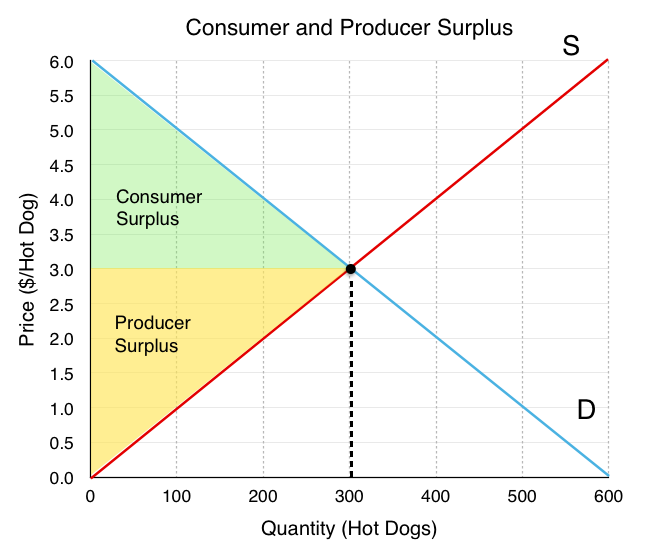
\includegraphics[width=6cm]{ts ex2.png}
    \end{figure}
    \end{itemize}
\end{frame}

\begin{frame}{CS/PS Solution 1}
    \begin{itemize}[<+->]
        \item In both cases, the base of the triangle is 300
        \item Consumer surplus is given by 
        $$CS=\frac{1}{2}(300)(6-3)=(150)(3)=450$$
        \item Producer Surplus is given by
        $$PS=\frac{1}{2}(300)(3-0)=150(3)=450$$
        \item Therefore, the total surplus 
        $$TS=CS+PS=450+450=900$$
    \end{itemize}
\end{frame}


\begin{frame}{CS/PS Exercise 2}
    \begin{itemize}
        \item Recall that the area of a triangle is $\frac{1}{2}$ base times height
        \item Compute consumer, producer, and total surplus for the market below. Assume supply and demand intersect at $Q^{*}=30$
    \begin{figure}
        \centering
        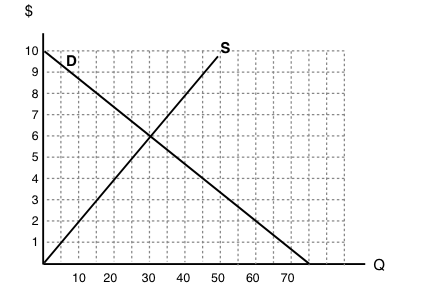
\includegraphics[width=6cm]{ts ex3.png}
    \end{figure}
    \end{itemize}
\end{frame}

\begin{frame}{CS/PS Solution}
    \begin{itemize}[<+->]
        \item In both cases, the base of the triangle is 30
        \item Consumer surplus is given by 
        $$CS=\frac{1}{2}(30)(10-6)=15(4)=60$$
        \item Producer Surplus is given by
        $$PS=\frac{1}{2}(30)(6-0)=15(6)=90$$
        \item Therefore, the total surplus 
        $$TS=CS+PS=60+90=150$$
    \end{itemize}
\end{frame}

\begin{frame}{CS/PS Challenge}
    \begin{itemize}
    \item Recall that the area of a triangle is $\frac{1}{2}$ base times height
        \item Compute consumer, producer, and total surplus in the market for coffee
    \begin{figure}
        \centering
        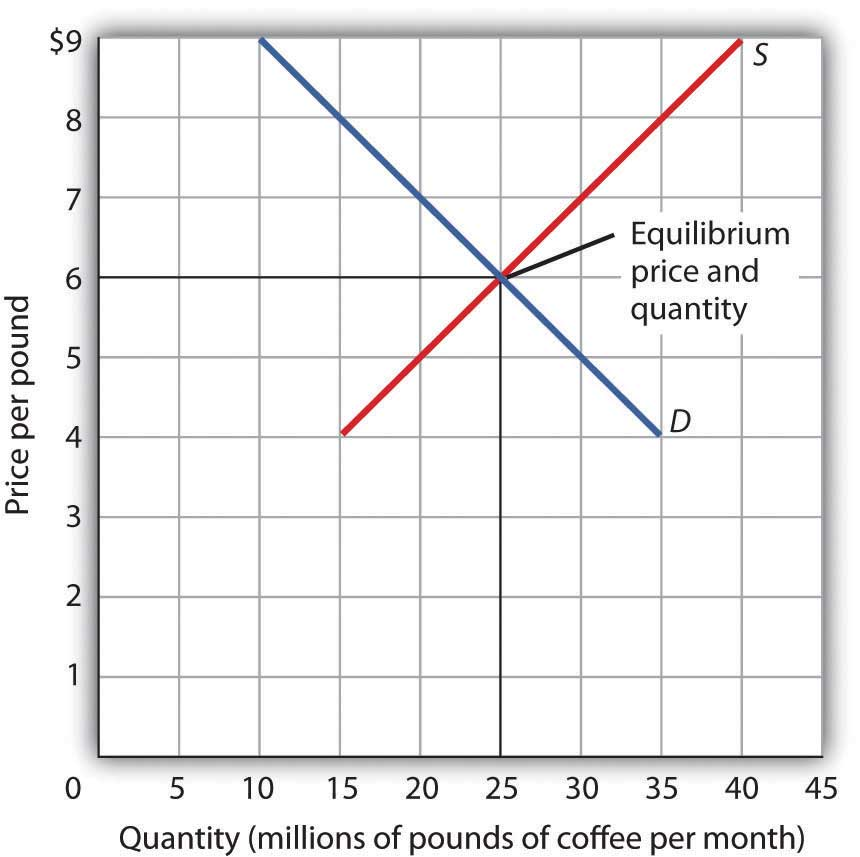
\includegraphics[width=6cm]{ts challenge.jpg}
    \end{figure}
    \end{itemize}
\end{frame}

\begin{frame}{CS/PS Challenge Solution}
    \begin{itemize}[<+->]
        \item You can use the method described in the previous set of slides to derive the $y$-intercept for supply and demand, which I strongly recommend you are familiar with
        \item In this case (which may not always be the case), we can look at the picture and see that the $y$-intercept for supply is 1, and for demand, is 11
        
        \item Consumer surplus is given by 
        $$CS=\frac{1}{2}(25)(11-6)=\frac{1}{2}(150)=75$$
        \item Producer Surplus is given by
        $$PS=\frac{1}{2}(25)(6-1)=\frac{1}{2}(150)=75$$
        \item Therefore, the total surplus 
        $$TS=CS+PS=75+75=150$$
    \end{itemize}
\end{frame}


\section*{Total Surplus}

\begin{frame}{Total Surplus}
    \begin{itemize}[<+->]
        \item For now, \underline{\textbf{Total Surplus}} is the sum of consumer and producer surplus
        \item A market is said to be \underline{\textbf{efficient}} if it maximizes total surplus
        \item Put another way, an allocation of resources in a market is said to be \underline{\textit{more efficient}} than another (in the same market)
        \item What's an allocation of resources?
        \begin{itemize}
            \item By this, we just mean who gets what in the economy
            \begin{itemize}
                \item Notice that, in a market equilibrium, there are some people who value a good, but who may not buy, because their WTP is below equilibrium price
                \item Likewise, some seller's may ``want" to sell, but their WTA is above market price 
            \end{itemize}
        \end{itemize}
    \end{itemize}
\end{frame}

\begin{frame}{The Social Planner}
    \begin{itemize}[<+->]
        \item The book describes a ``benevolent social planner", a dictator whose sole interest is maximizing welfare
        \item Mankiw doesn't go into many of the specifics, but here is one version:
        \begin{itemize}
            \item The social planner knows the valuations on behalf of both consumers and producers
            \item The social planner decides exactly which producers produce, and which consumers will get the goods
            \item The planner then takes money from the consumers, gives them the good, and then distributes the money to the producers who produced
            \item If we assume, for simplicity, that the planner must charge the same amount across consumers, then we get a market price
        \end{itemize}
        \item Keep in mind that as that as the price goes up, producers are better off (PS$\uparrow$) but consumers are worse off (CS$\downarrow$), and vice versa\footnote{\vspace{1mm}This is the only takeaway on this slide I want you to remember}
        \item Thus, based on valuations, the planner decides upon a market price, such that the total surplus in the market is maximized
    \end{itemize}
\end{frame}

\begin{frame}{Visualizing the Social Planner 1}
    \begin{itemize}[<+->]
        \item Suppose the social planner sets the price to be $\$2$ in the following market:
        \begin{figure}
            \centering
            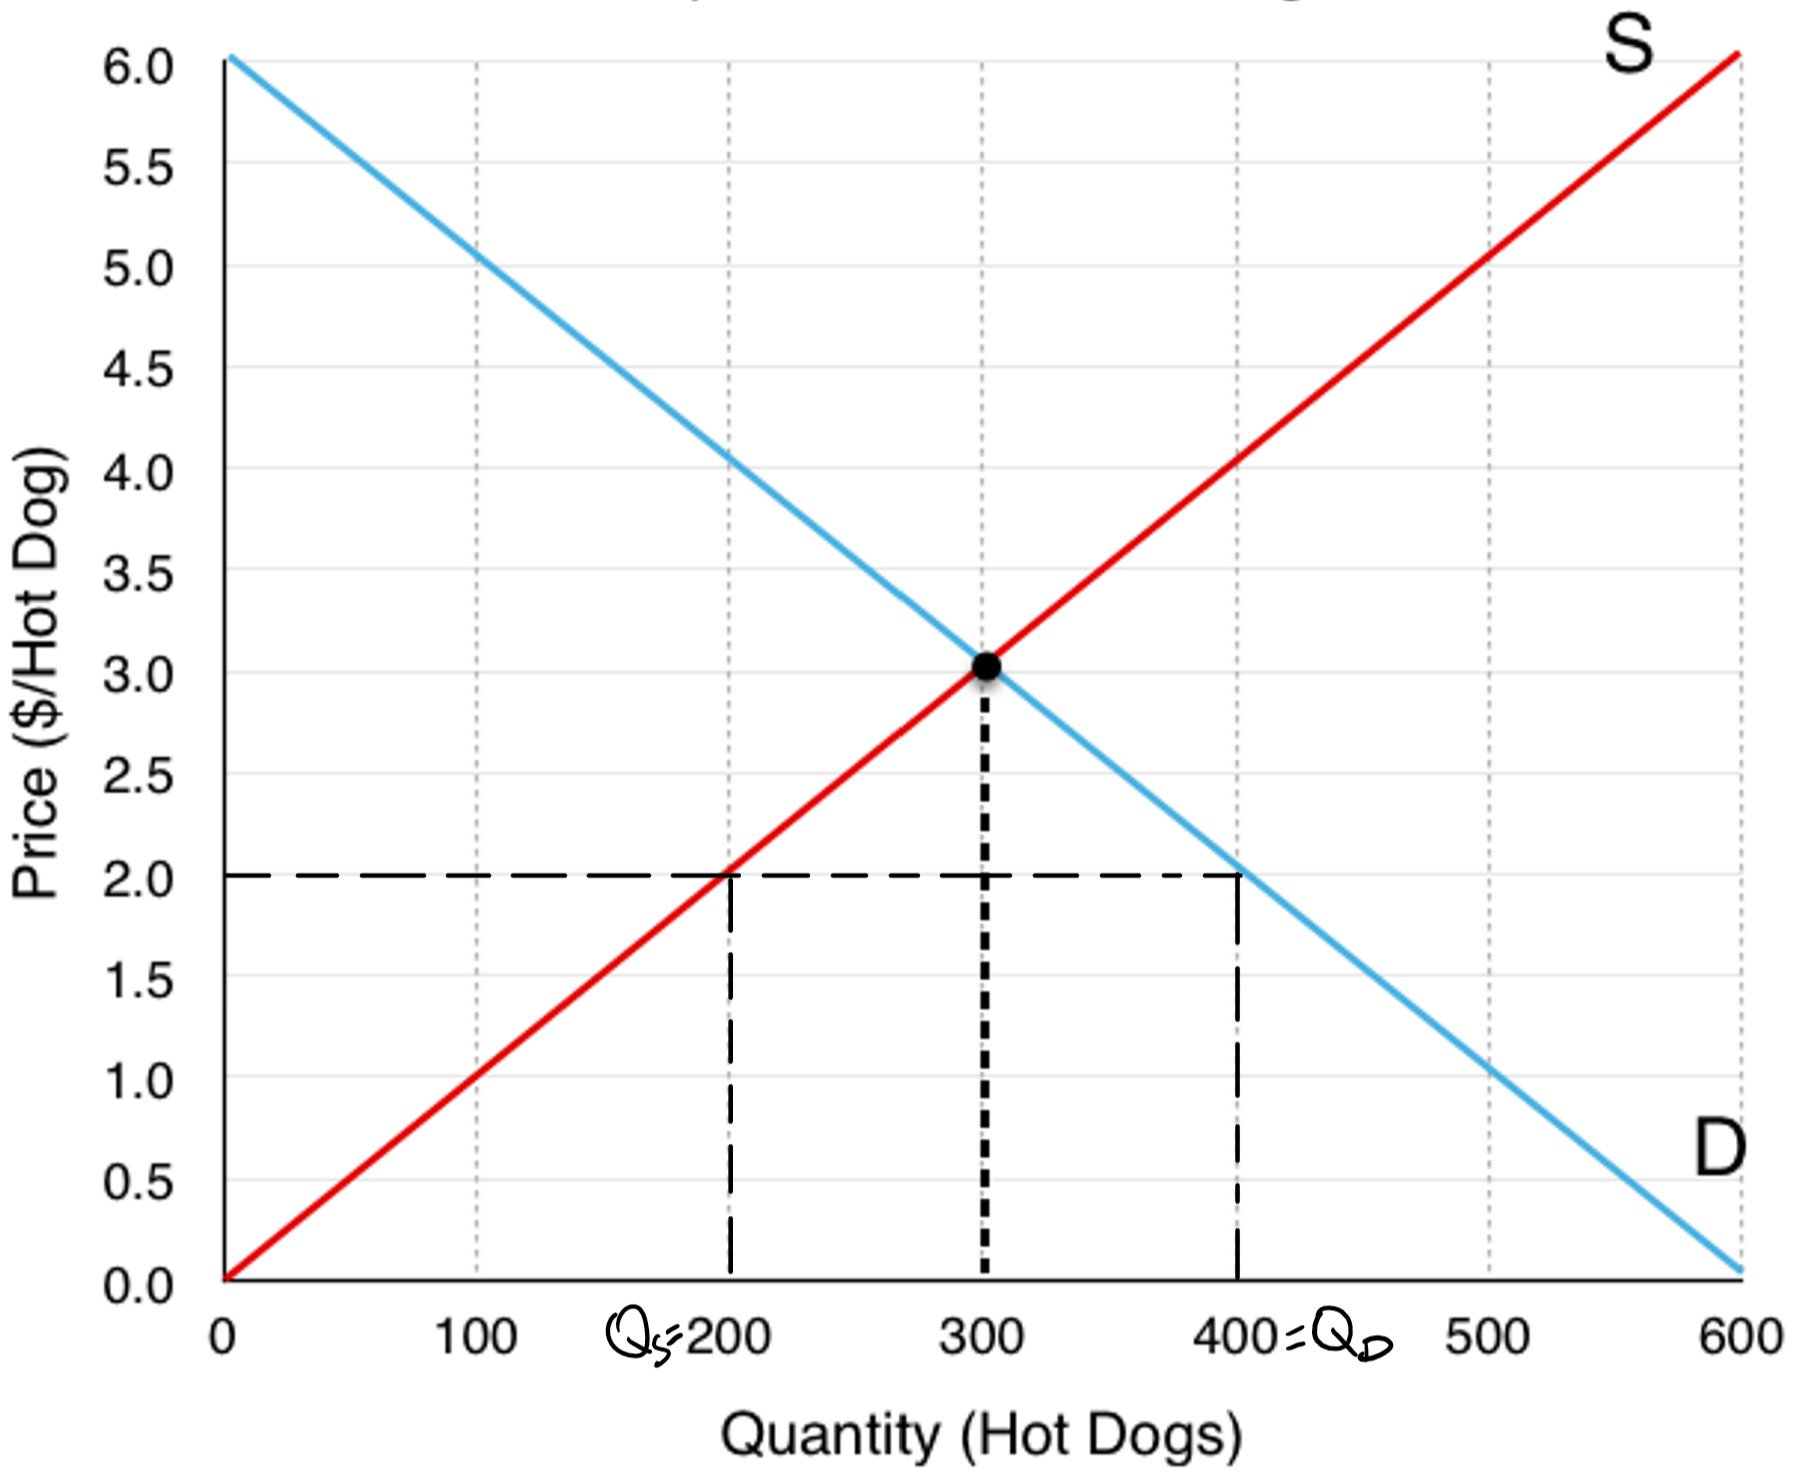
\includegraphics[width=5cm]{below market price.png}
        \end{figure}
        \item In this case, the quantity demanded is 400, while the quantity supplied is only 200
        \item So how many units get traded?
        \begin{itemize}
            \item Only 200, because only 200 people are willing to sell
        \end{itemize}
    \end{itemize}
\end{frame}

\begin{frame}{Visualizing the Social Planner 1 (cont.)}
    \begin{itemize}[<+->]
        \item So what are consumer and producer surpluses in this market?
        \begin{figure}
            \centering
            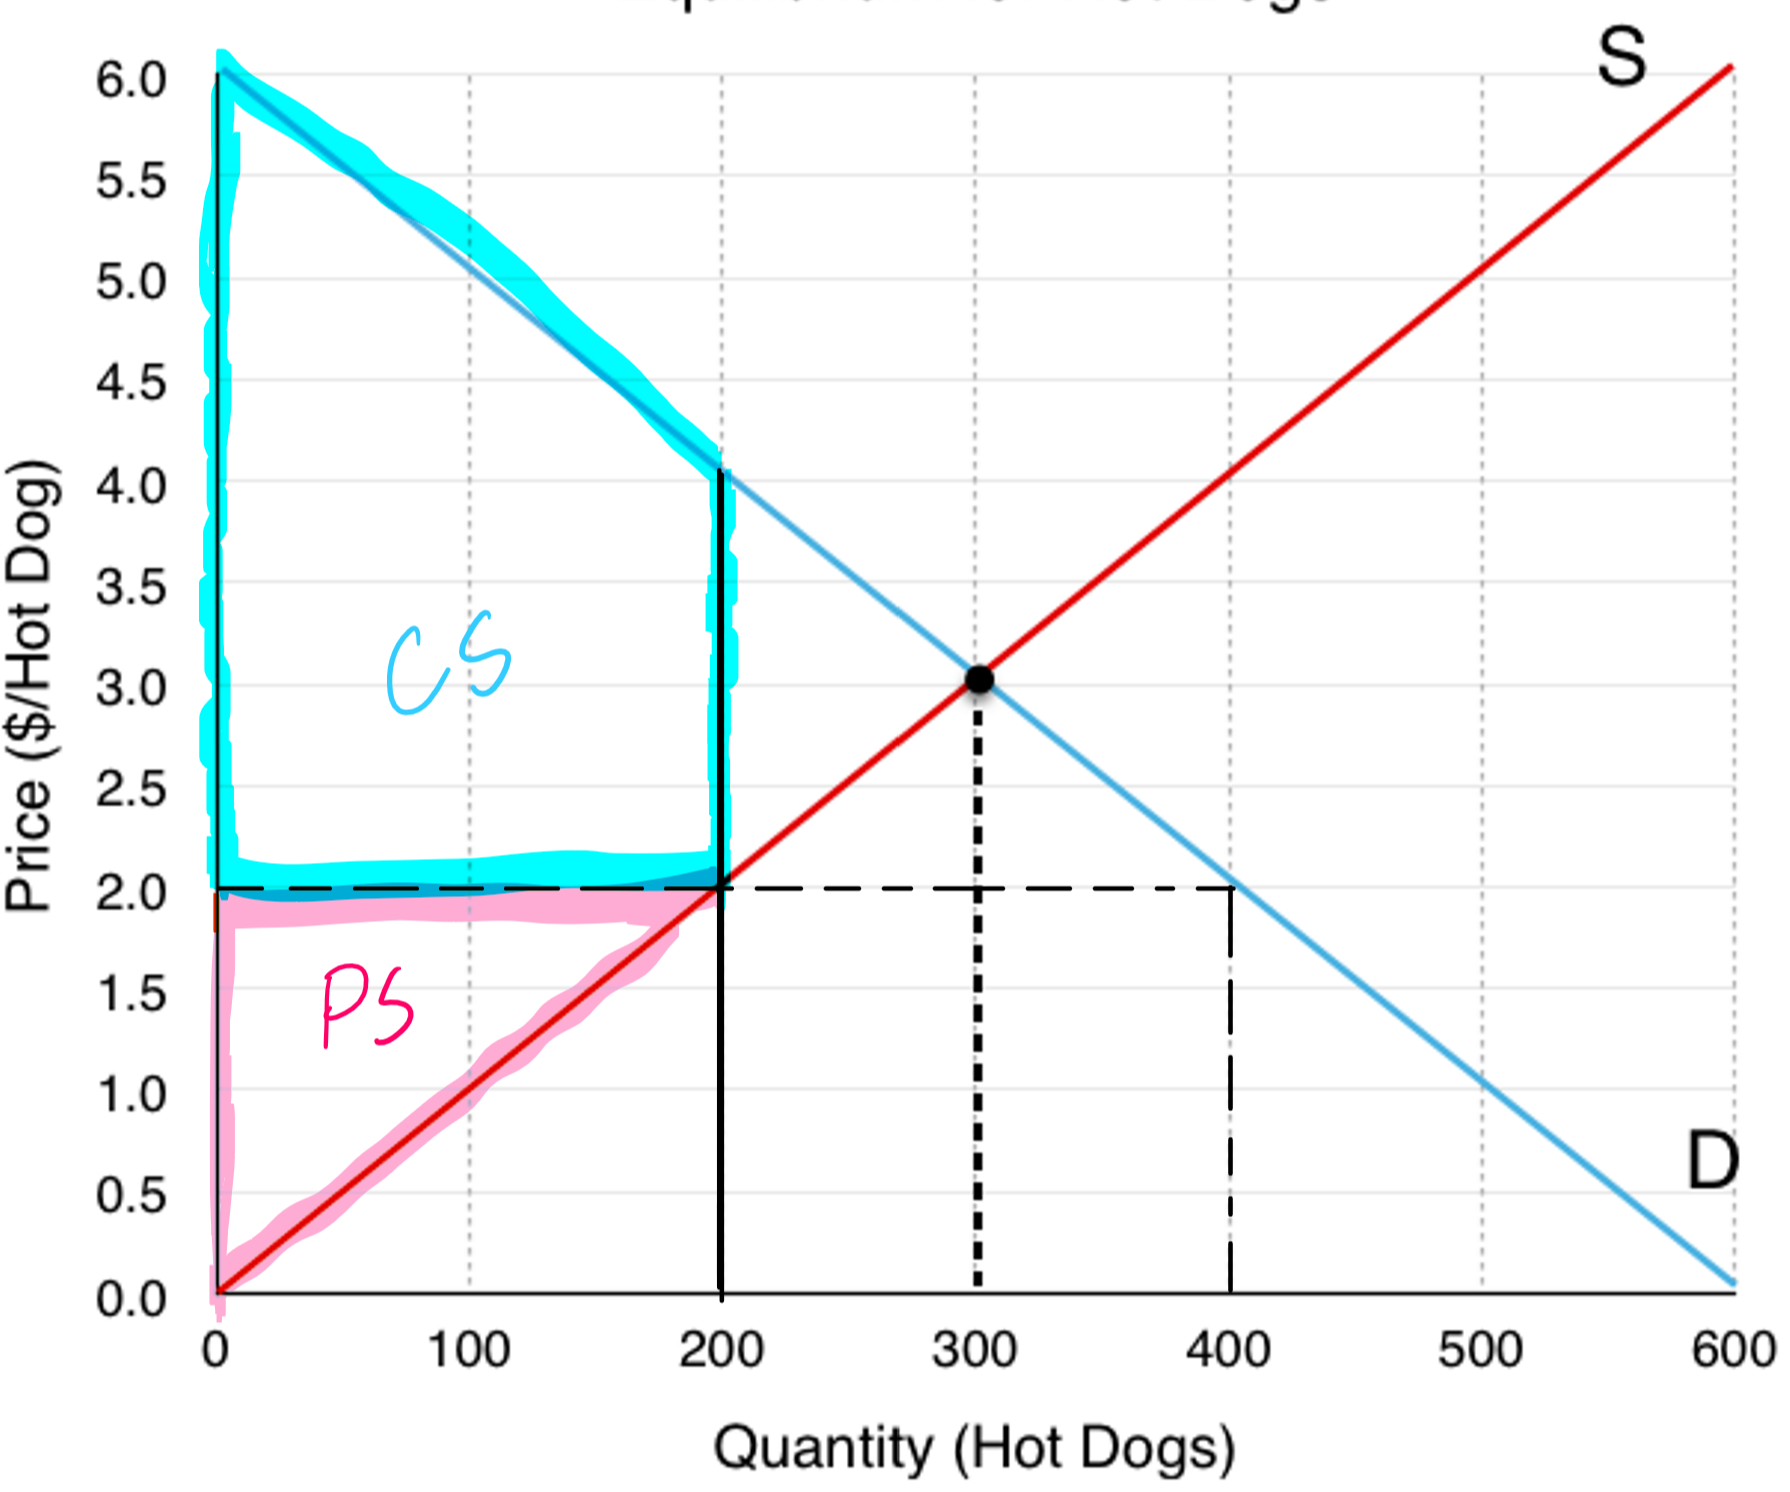
\includegraphics[width=5cm]{below market price cs-ps.png}
        \end{figure}
        \item Since the amount being traded is 200, we have to cut we have stop at $Q=200$; those other 200 demanders do not get the product, so their surplus is not counted
        \item Remember that CS is WTP (demand curve) - price, and PS is price - WTA (supply curve) 
    \end{itemize}
\end{frame}

\begin{frame}{Visualizing the Social Planner 1 (cont.)}
    \begin{itemize}[<+->]
        \item So what are consumer and producer surpluses in this market?\footnote{Note that you have to break up CS into a rectangle and a triangle, to get the area}
        \begin{figure}
            \centering
            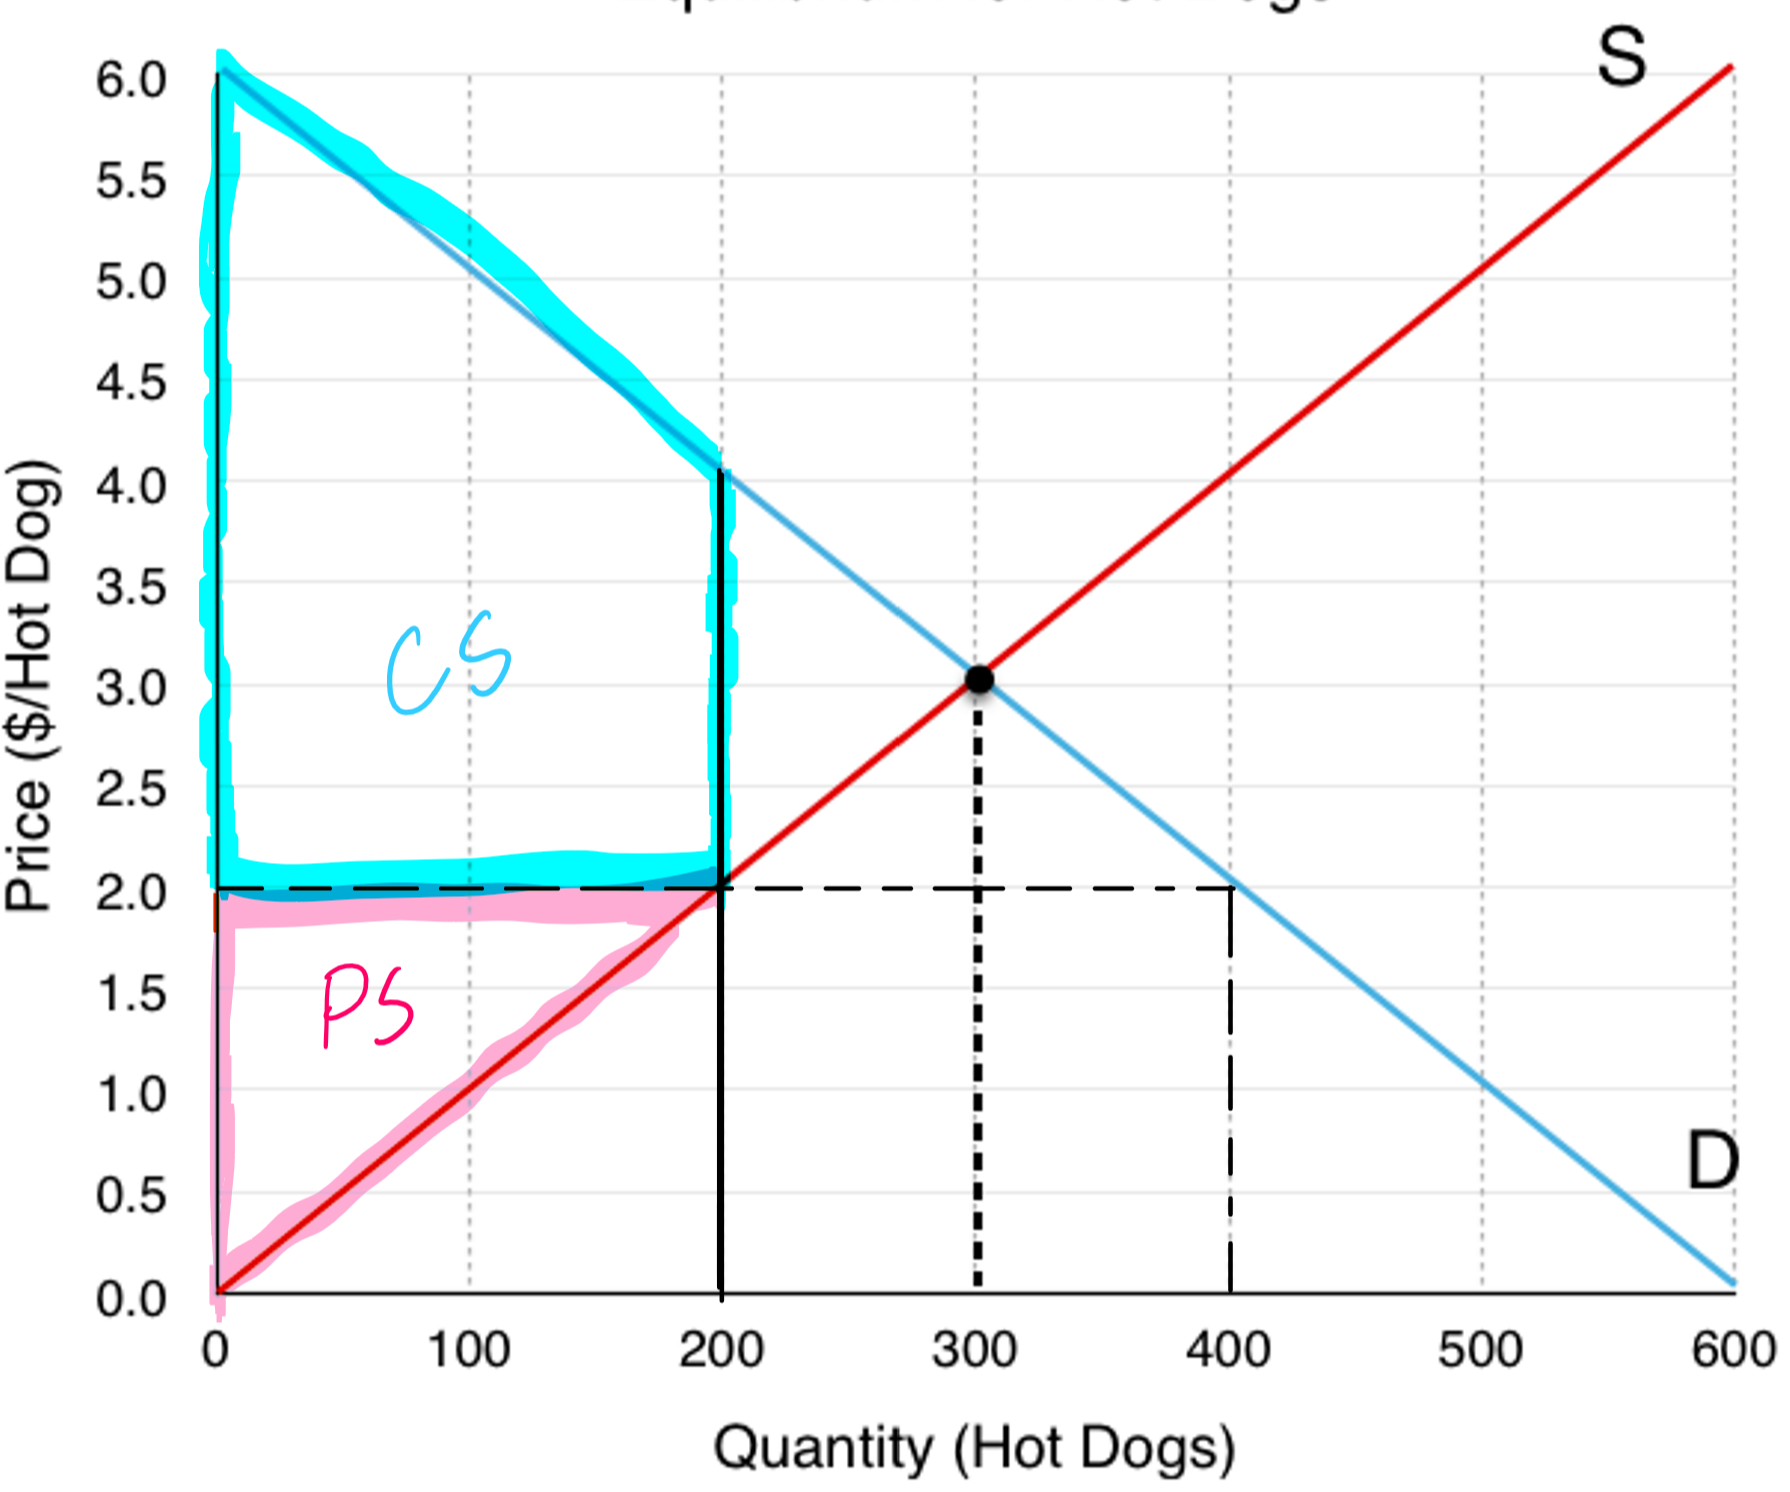
\includegraphics[width=5cm]{below market price cs-ps.png}
        \end{figure}
    \end{itemize}
        \begin{align*}
            PS&=(1/2)(200)(2)=200\\
            CS&=\underbrace{(1/2)(200)(6-4)}_{{Triangle}} + \underbrace{(200)(4-2)}_{Rectangle}=(100)(2) + (200)(2)=600
        \end{align*}
\end{frame}

\begin{frame}{Visualizing the Social Planner 1 (conclusion)}
    \begin{itemize}[<+->]
        \item As we can see, consumers who were allotted the product benefited greatly
        \item However, 200 consumers valued the product at greater than or equal to the price, but didn't get allocated a hot dog. Plus, producer surplus looks a little small
        \item Our TS in this case is 800
    \end{itemize}
\end{frame}

\begin{frame}{Visualizing the Social Planner 2}
    \begin{itemize}[<+->]
        \item Now suppose the social planner sets the price to be $\$5$ in the market:
        \begin{figure}
            \centering
            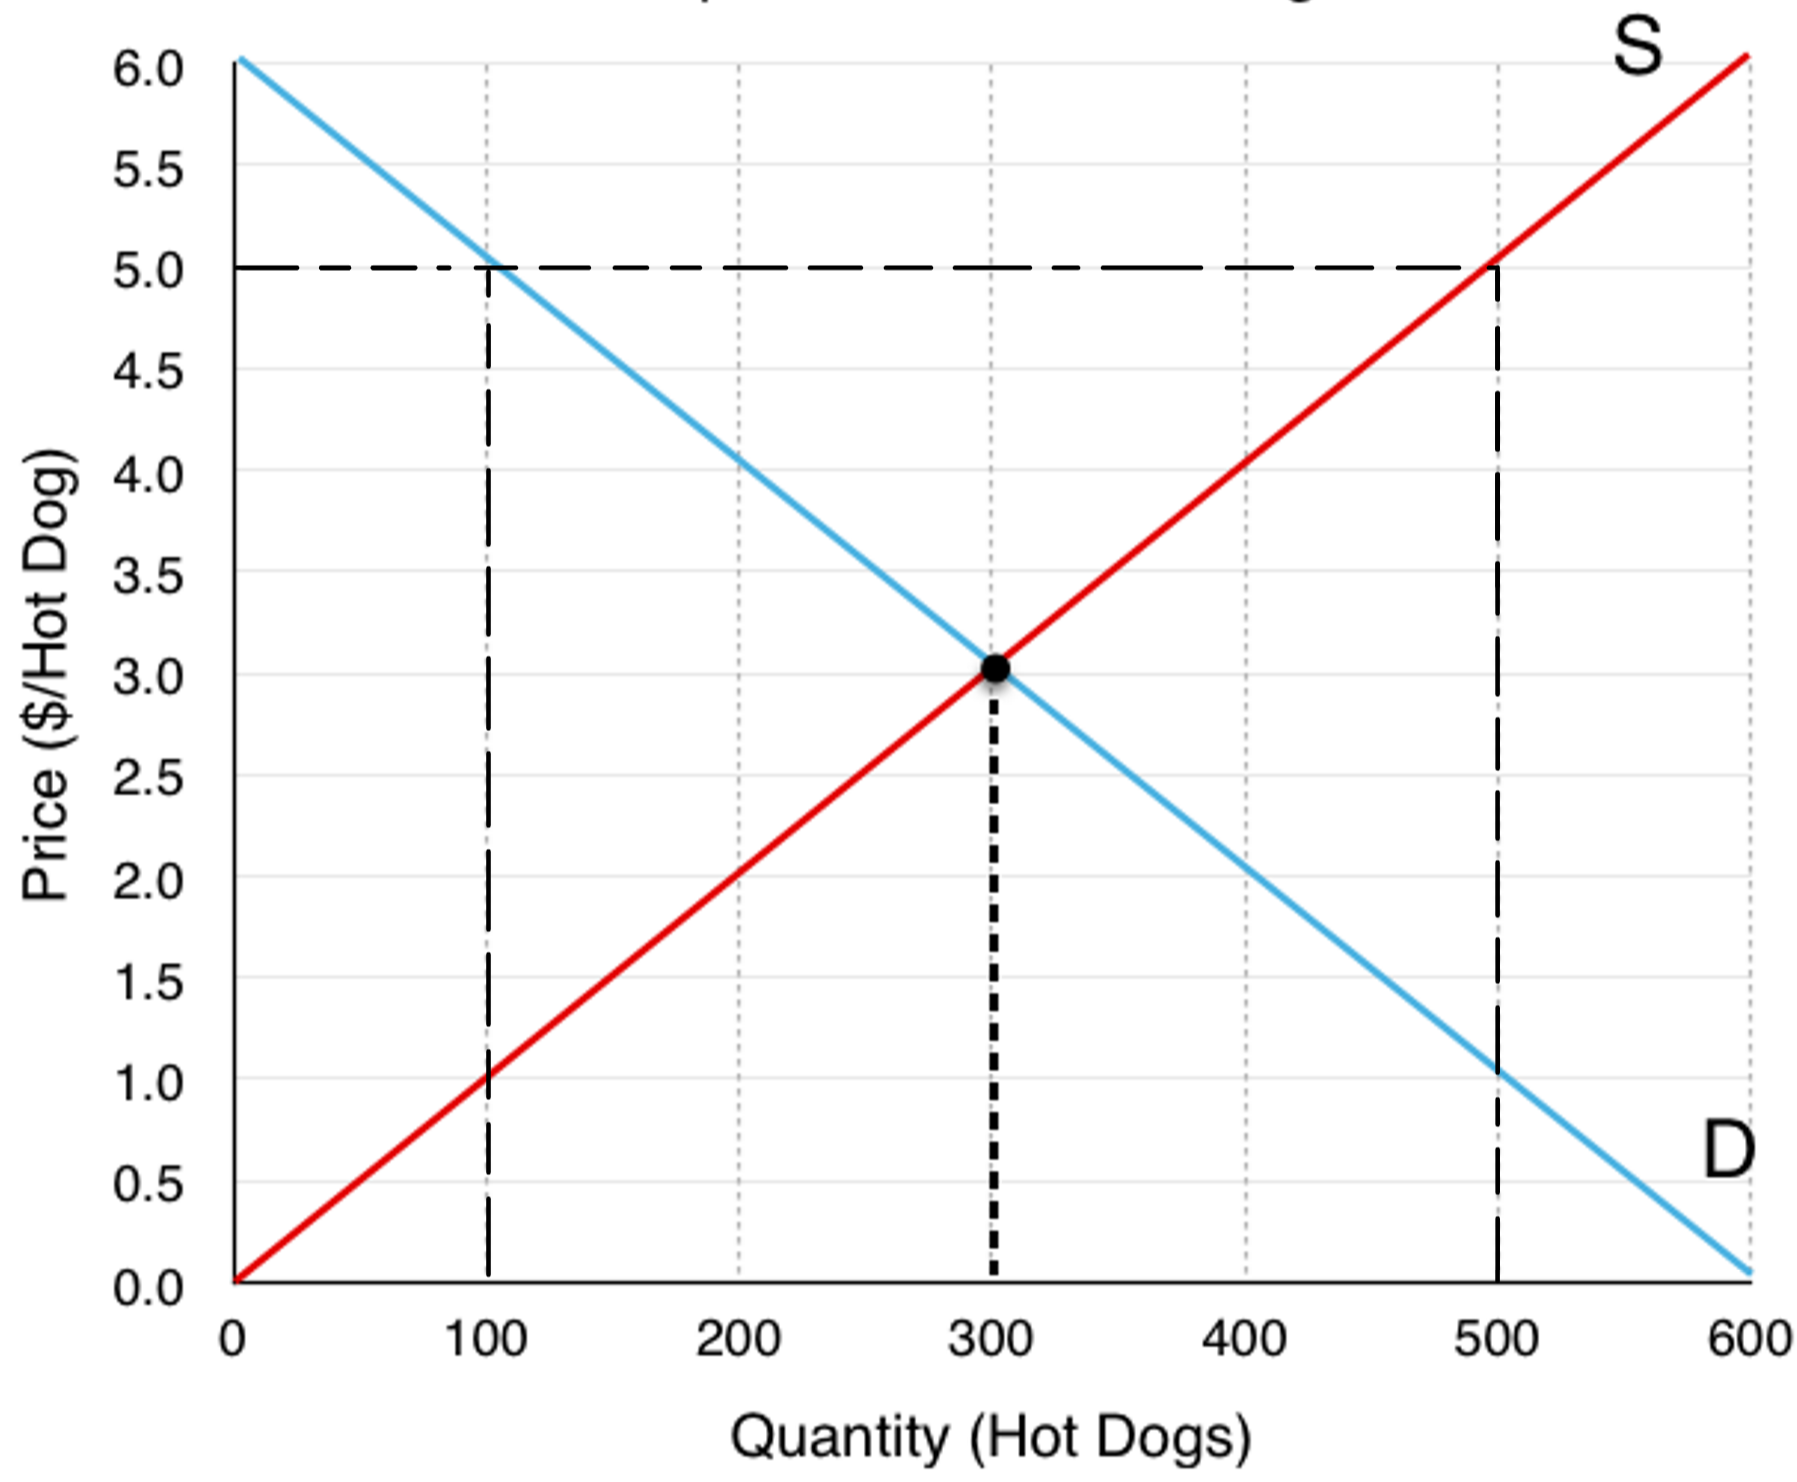
\includegraphics[width=5cm]{above market price.png}
        \end{figure}
        \item In this case, the quantity demanded is 100, while the quantity supplied is all the way at 500
        \item So how many units get traded?
        \begin{itemize}
            \item Only 100, because only 100 people value the product enough
        \end{itemize}
    \end{itemize}
\end{frame}


\begin{frame}{Visualizing the Social Planner 2 (cont.)}
    \begin{itemize}[<+->]
        \item So what are consumer and producer surplus now?
        \begin{figure}
            \centering
            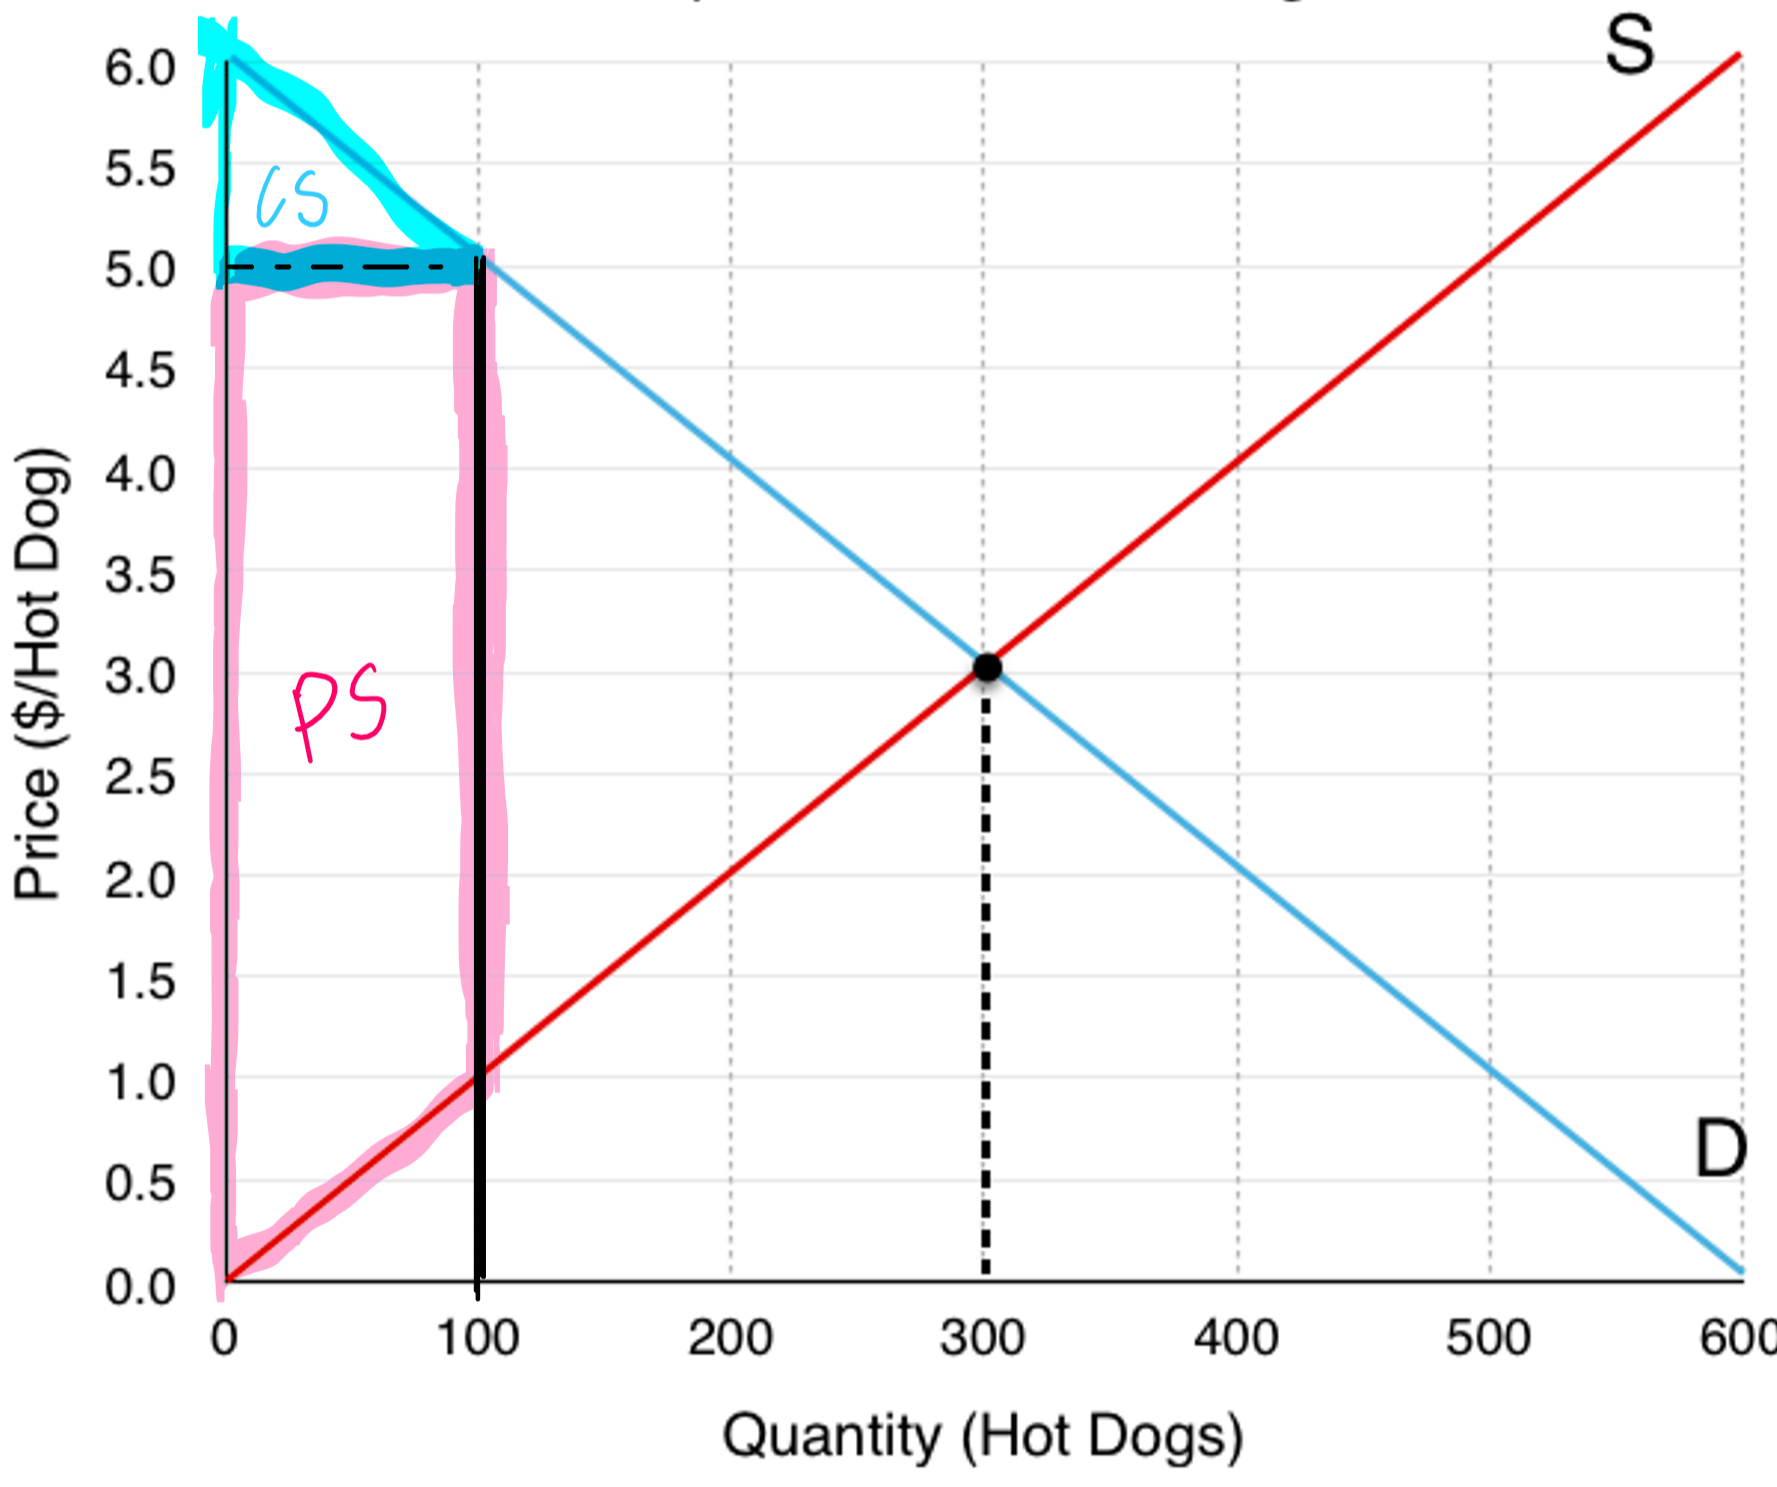
\includegraphics[width=5cm]{above market price cs-ps.png}
        \end{figure}
    \end{itemize}
        \begin{align*}
            CS&=(1/2)(100)(1)=50\\
            PS&=\underbrace{(1/2)(100)(1)}_{{Triangle}} + \underbrace{(100)(5-1)}_{Rectangle}=50 + 400=450
        \end{align*}
\end{frame}

\begin{frame}{Visualizing the Social Planner 2 (conclusion)}
    \begin{itemize}[<+->]
        \item As we can see, producers who were told to produce and ``sell" the product benefited greatly
        \item However, 400 producers were willing to spend the time producing the product to sell it for $\$5$ to the social planner, but didn't get to; also, CS is low
        \item Our TS in this case is 500
        \item This is less than before, only by chance: if I had said the price was $\$4$, we would get the same TS
        \item Nonetheless, we would say that the first allocation of resources is \textit{more efficient} than this one, because the old TS was 800, and the new TS is only 500
    \end{itemize}
\end{frame}


\begin{frame}{Visualizing the Social Planner 3}
    \begin{itemize}[<+->]
        \item Now suppose the social planner sets the price to be $\$3$ in the market:
        \begin{figure}
            \centering
            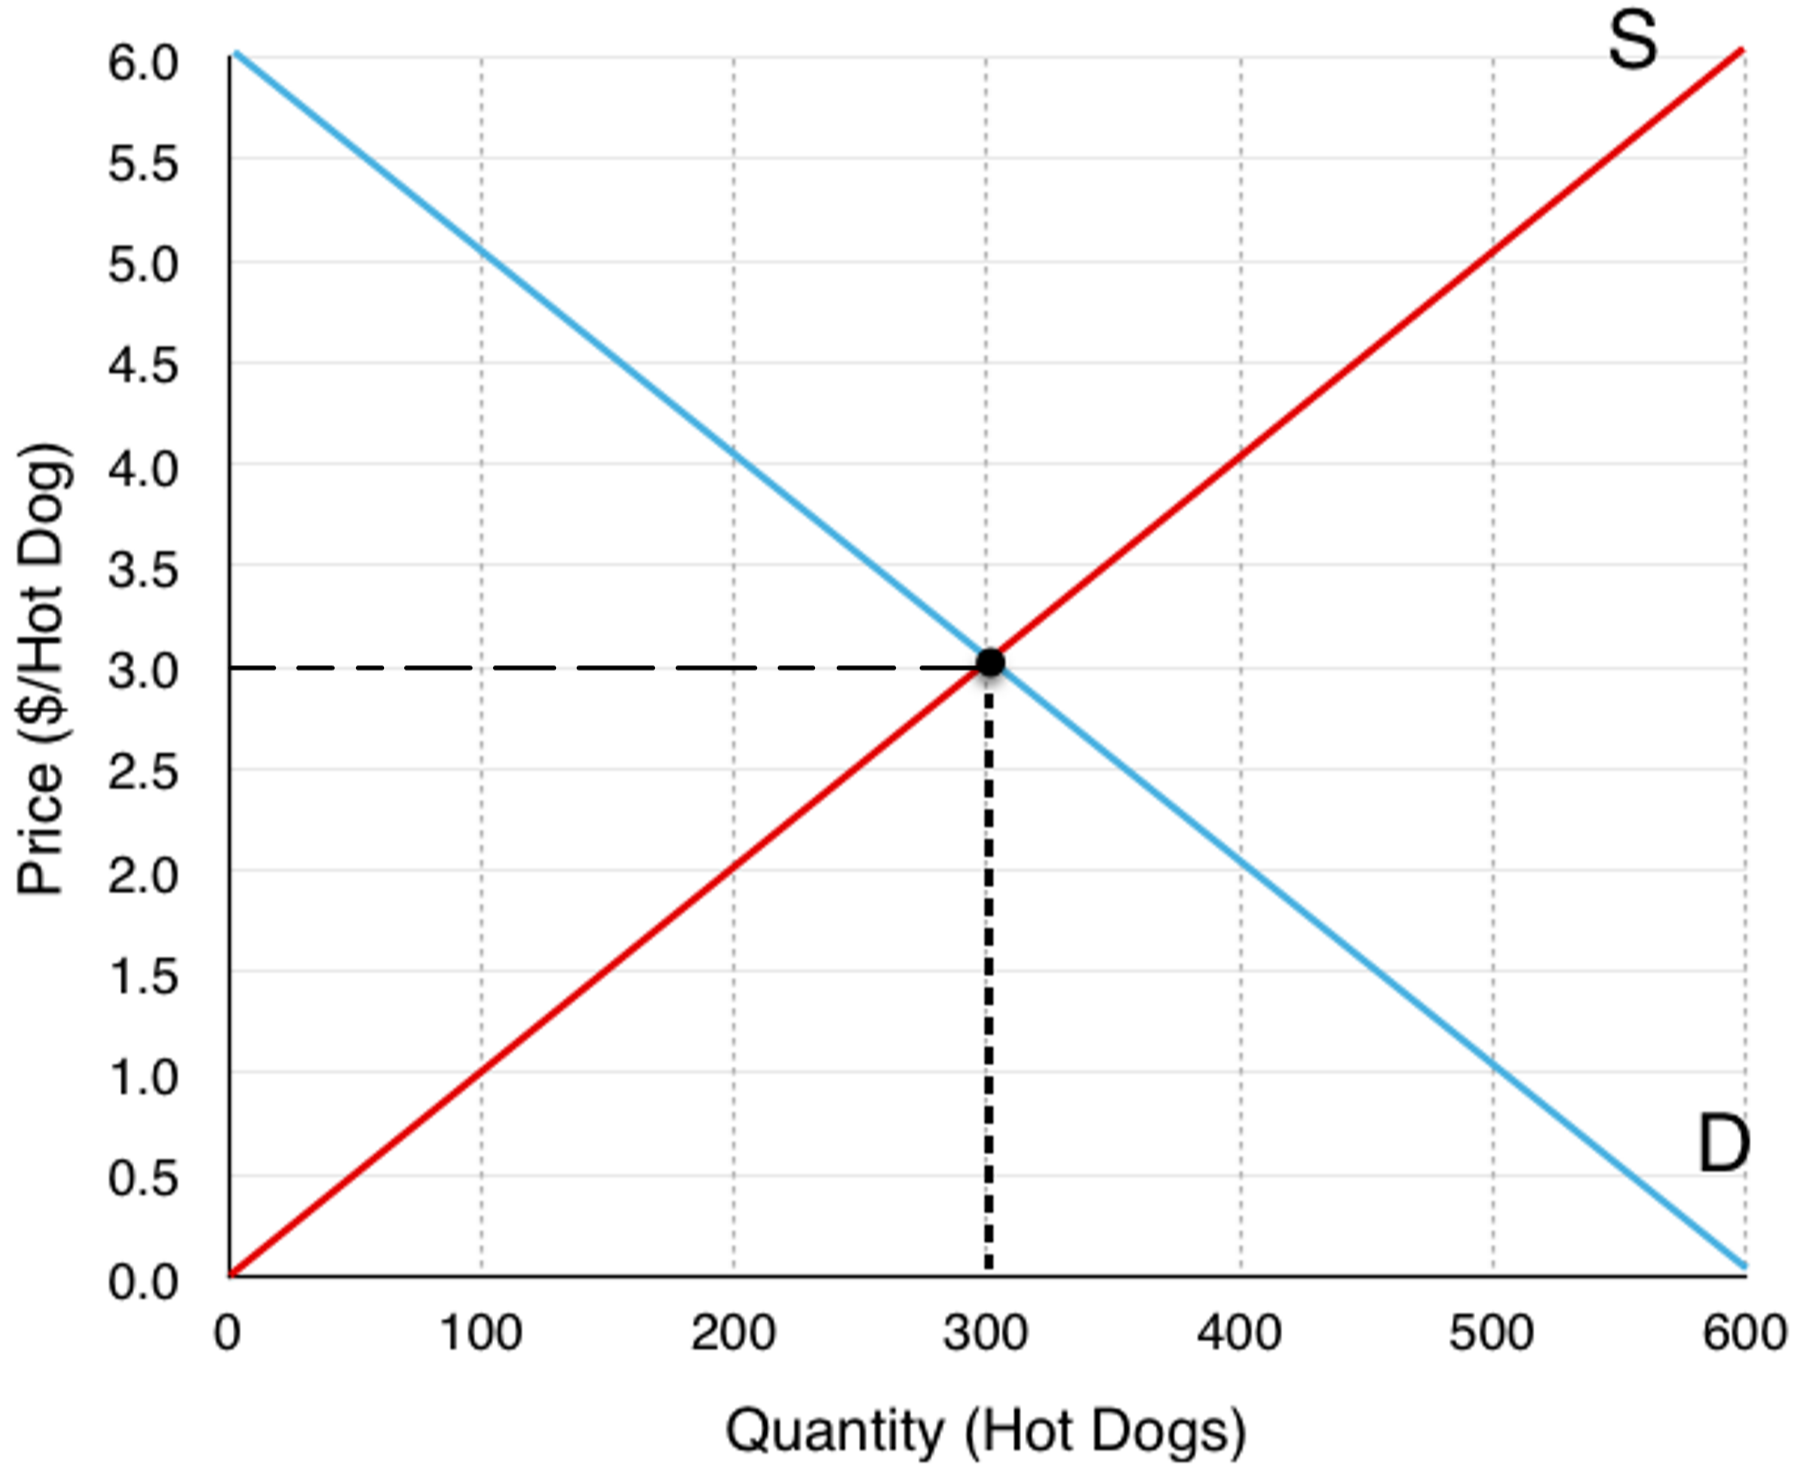
\includegraphics[width=5cm]{at market price.png}
        \end{figure}
        \item In this case, the quantity demanded and quantity supplied are both 300
    \end{itemize}
\end{frame}


\begin{frame}{Visualizing the Social Planner 3 (cont.)}
    \begin{itemize}[<+->]
        \item So what are consumer and producer surplus now?
        \begin{figure}
            \centering
            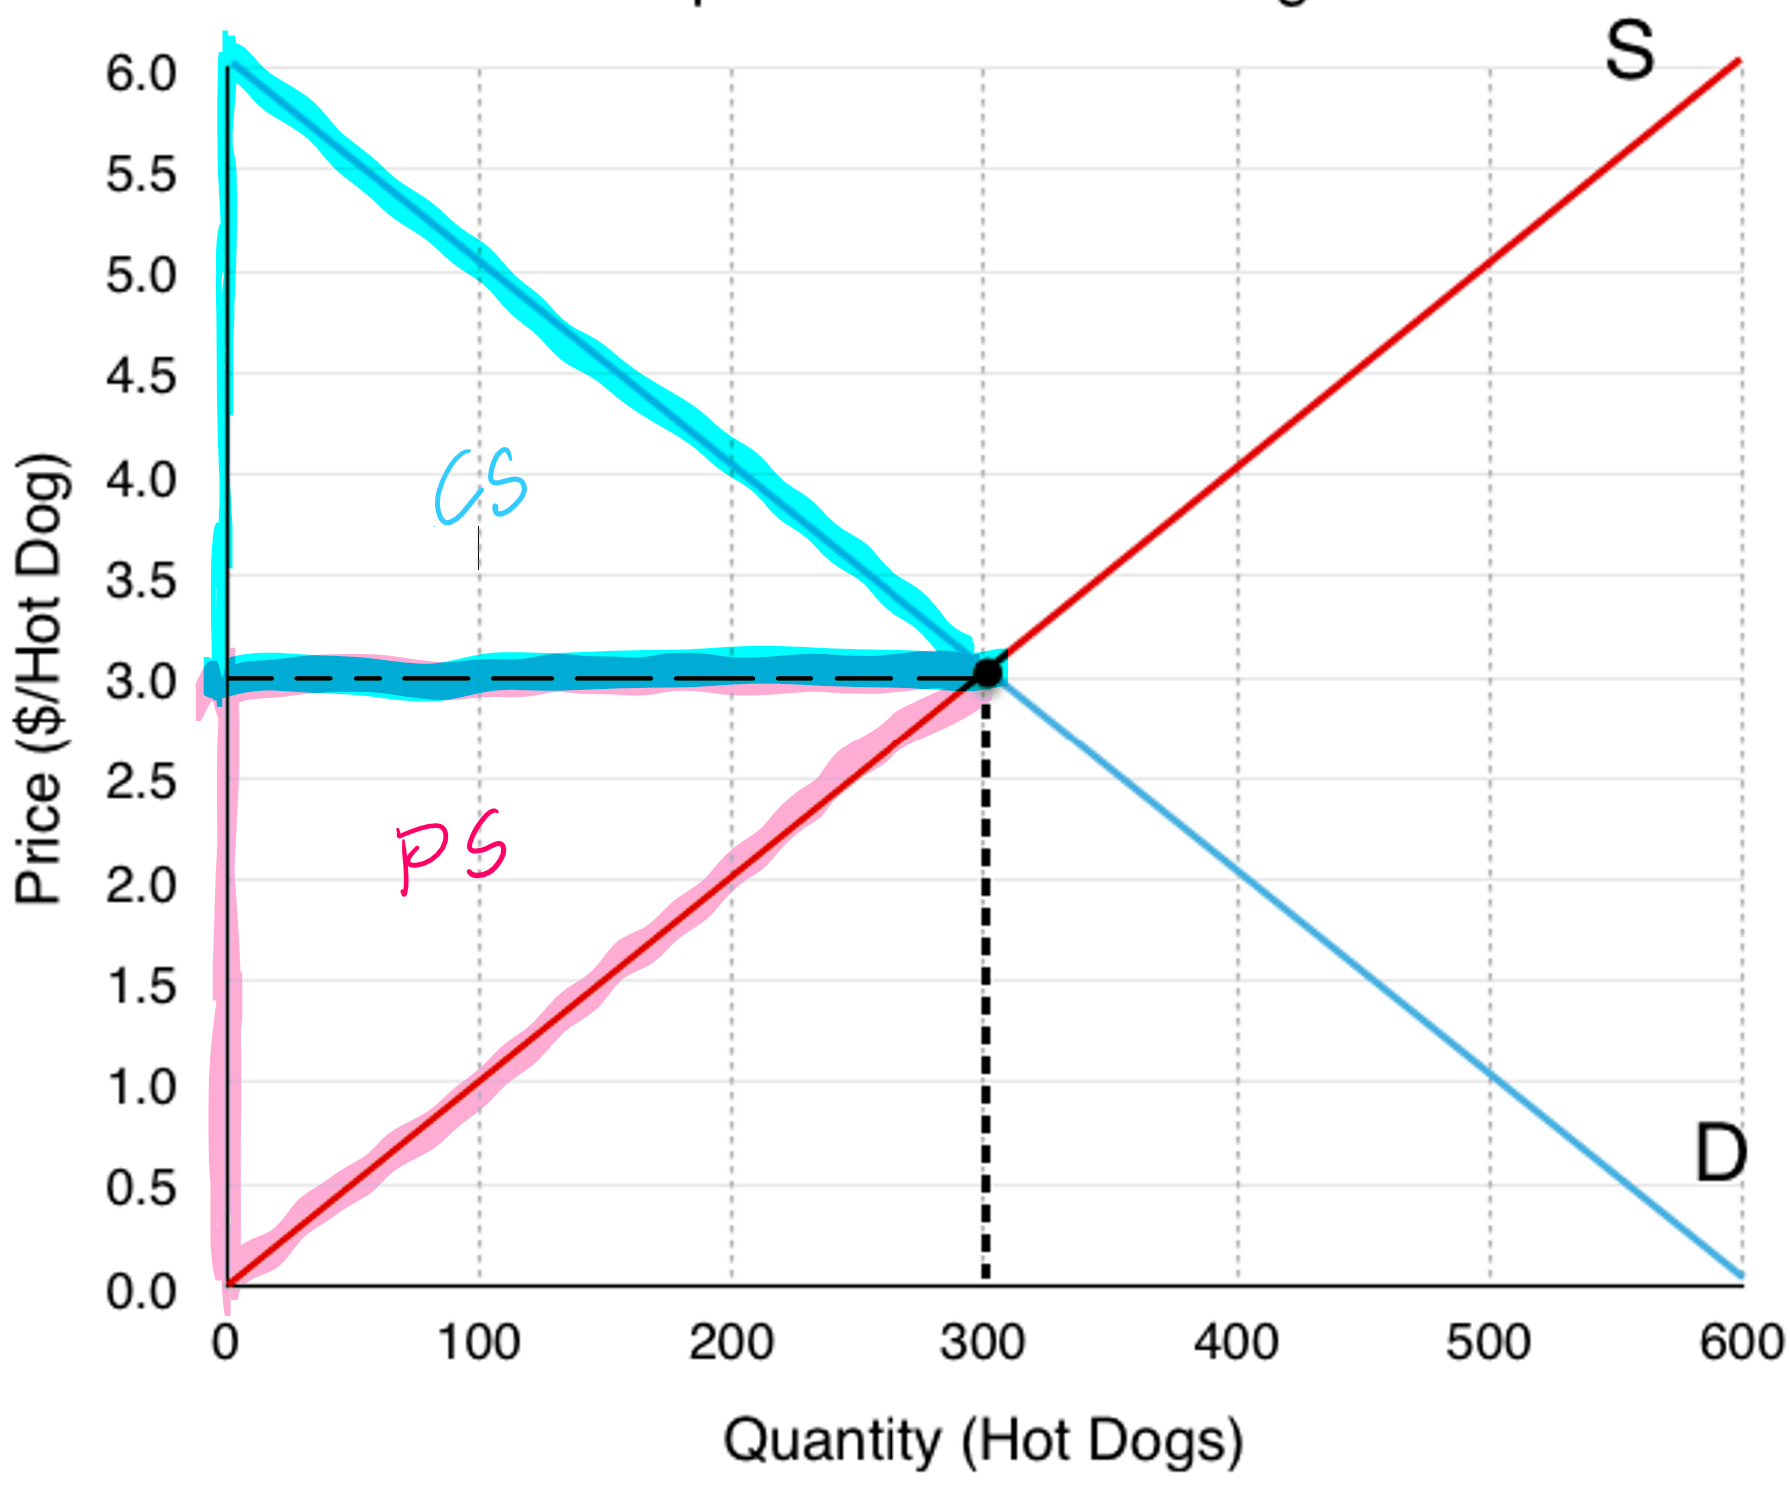
\includegraphics[width=5cm]{at market price cs-ps.png}
        \end{figure}
    \end{itemize}
        \begin{align*}
            CS&=(1/2)(300)(6-3)=150(3)=450\\
            PS&=(1/2)(300)(3-0)=150(3)=450
        \end{align*}
\end{frame}

\begin{frame}{Visualizing the Social Planner 3 (conclusion)}
    \begin{itemize}[<+->]
        \item Now, nobody who values consuming the good above market price or producing the good below market price is excluded
        \item Moreover, our TS is 900, the highest so far
        \item Not only is this allocation \textit{more efficient} than the other two, but it is the \underline{efficient} allocation, because the market equilibrium maximizes total surplus
        \item The social planner is not something I need you to know, but I would like you to understand efficiency
        \begin{itemize}
            \item The way Mankiw describes the planner is akin to just making the market mechanism into a person, other versions of the social planner can be more interesting, but are outside the scope of this class
        \end{itemize}
    \end{itemize}
\end{frame}




\begin{frame}{Summary of Welfare Economics}
    \begin{itemize}[<+->]
        \item Demand is a reflection of consumers' willingness to pay -- the maximum amount they would pay for a product
        \item Supply is a reflection of producers' willingness to accept -- the maximum amount they would sell for a product for
        \begin{itemize}
            \item Each of these has a ``Total" definition, for when we want to talk about the net quantity being bought or sold, and a ``marginal" definition, when we want to talk about only the \textit{next} product being bought/sold
        \end{itemize}
        \item These notions of supply and demand generate two regions, graphically:
        \begin{itemize}
            \item The region between market price and WTP (reflected through the demand curve), known as consumer surplus 
            \item The region between market price and WTA (reflected through the supply curve), known as producer surplus
        \end{itemize}
        \item The sum of consumer and producer surplus is known as \underline{Total Surplus}, and a market is known as ``efficient" if it maximizes total surplus
    \end{itemize}
\end{frame}

\section*{Intro to Price Controls}

\begin{frame}{Below-Equilibrium Price}
    \begin{itemize}[<+->]
        \item Consider the previous social planner examples, but without the lens of the social planner (i.e., we are just imagining that the price is not in equilibrium)
        \begin{figure}
            \centering
            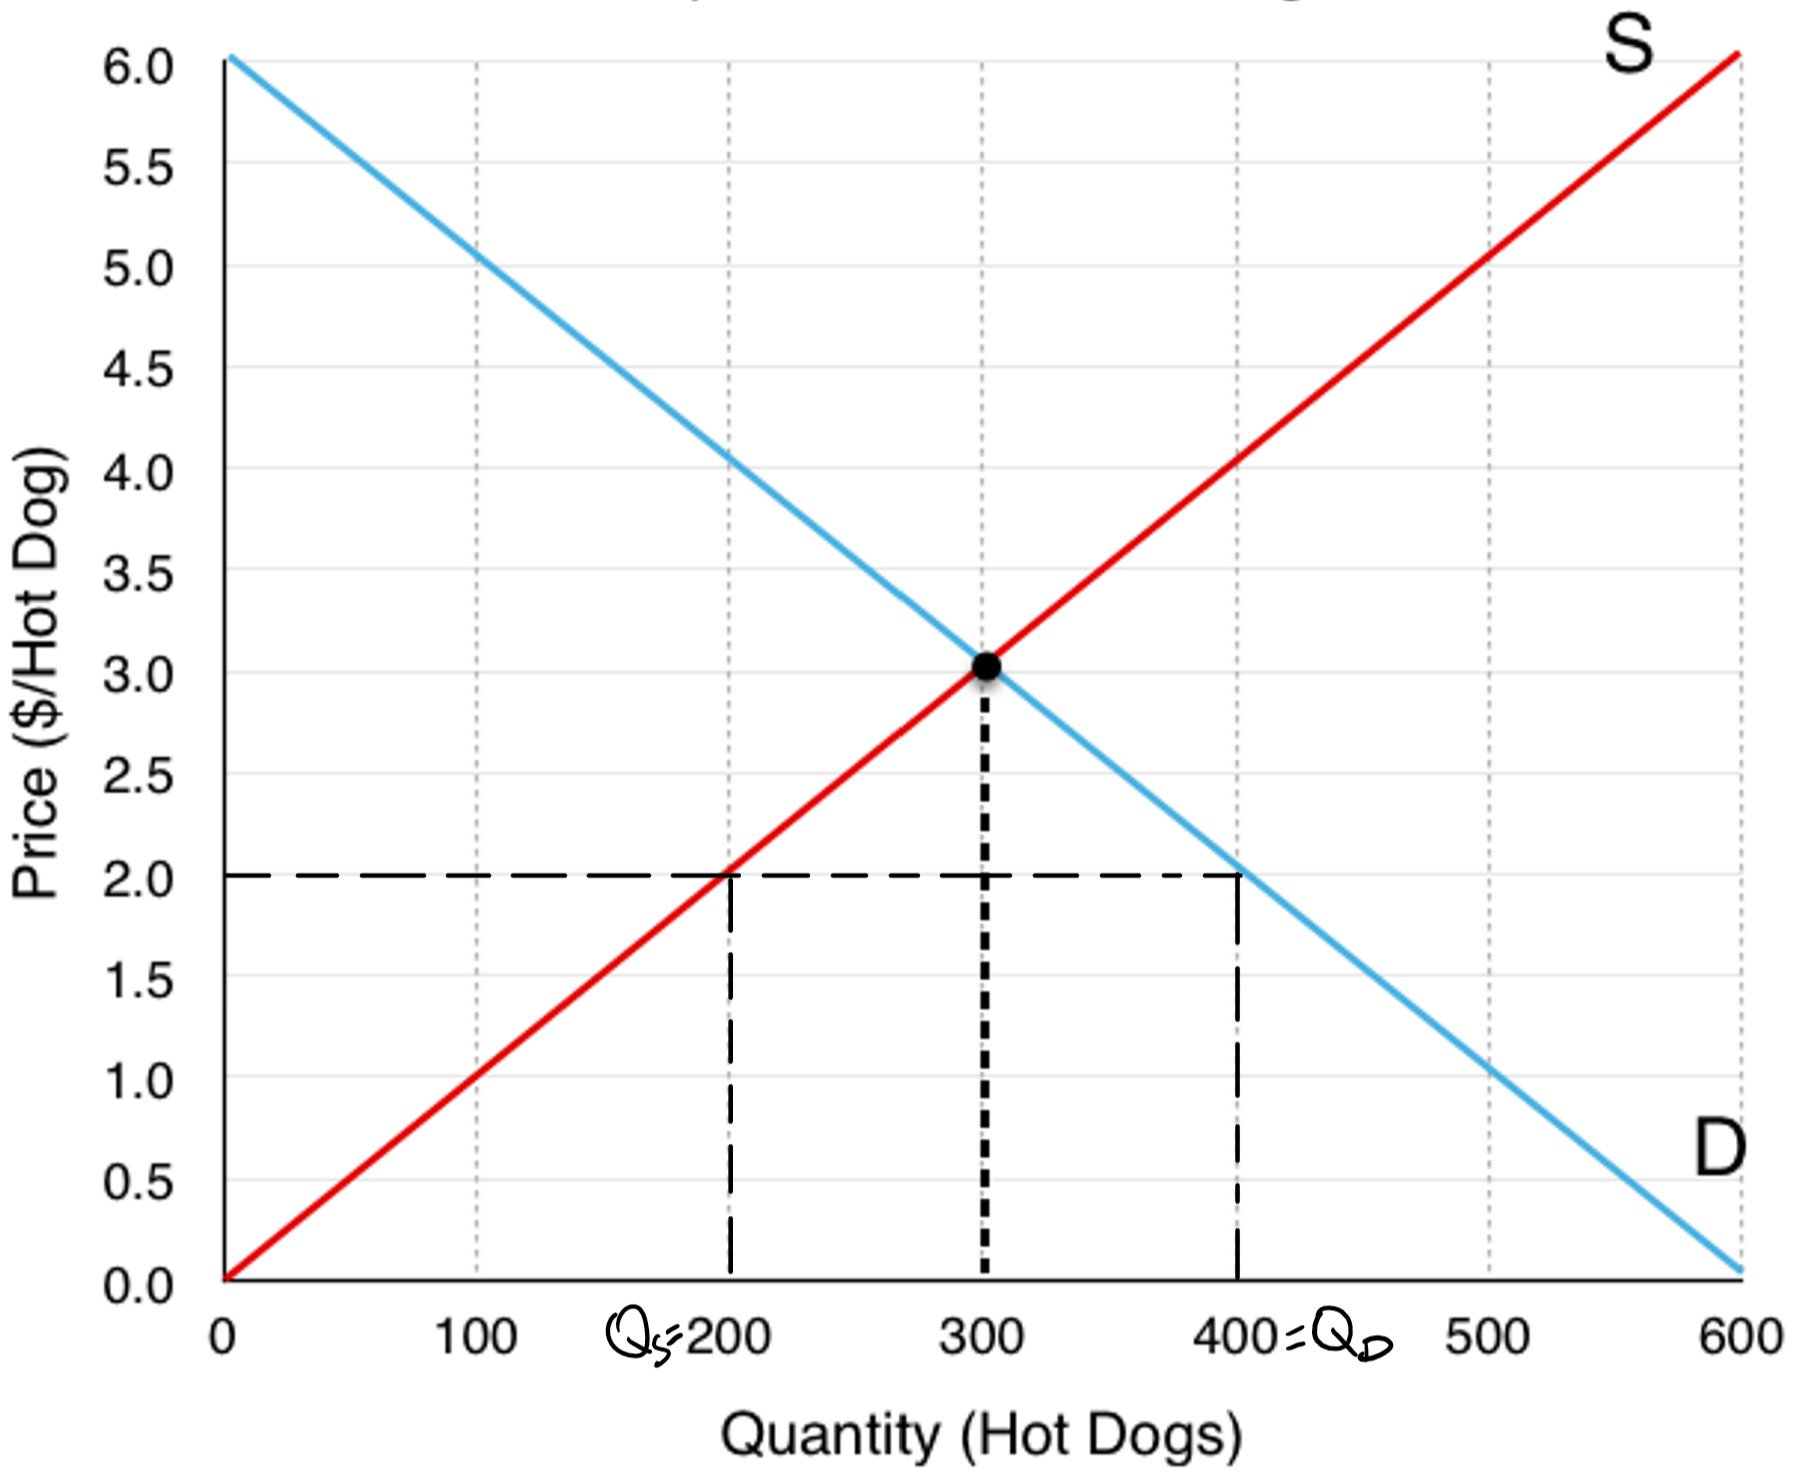
\includegraphics[width=5cm]{below market price.png}
        \end{figure}
        \item In this case, the quantity demanded is 400, while the quantity supplied is only 200. What is this called in a market setting?
        \item A \underline{shortage}, because the quantity demanded exceeds the quantity supplied
    \end{itemize}
\end{frame}

\begin{frame}{A Shortage}
    \begin{itemize}[<+->]
        \item In general, consumers like lower prices, and producers like higher prices
        \item That is, consumers are always willing and happy to go lower when negotiating a price, and producers are always willing to go higher
        \item So, when the price is below the equilibrium, such that there is a shortage, whose responsibility is it to raise the price?
        \begin{itemize}
            \item It's the \underline{consumers'} responsibility to increase the offer that they give to suppliers
            \item Technically, both parties are responsible for agreeing upon a (higher) price, but the offer to raise the price is always implicitly on the table for suppliers, because they benefit from it
        \end{itemize}
        \item Once consumers offer to pay more, the price rises, the size of the shortage (in our example: 200) falls, and we repeat until equilibrium
    \end{itemize}
\end{frame}

\begin{frame}{Above-Equilibrium Price}
    \begin{itemize}[<+->]
        \item What about when the price was $\$5$?
        \begin{figure}
            \centering
            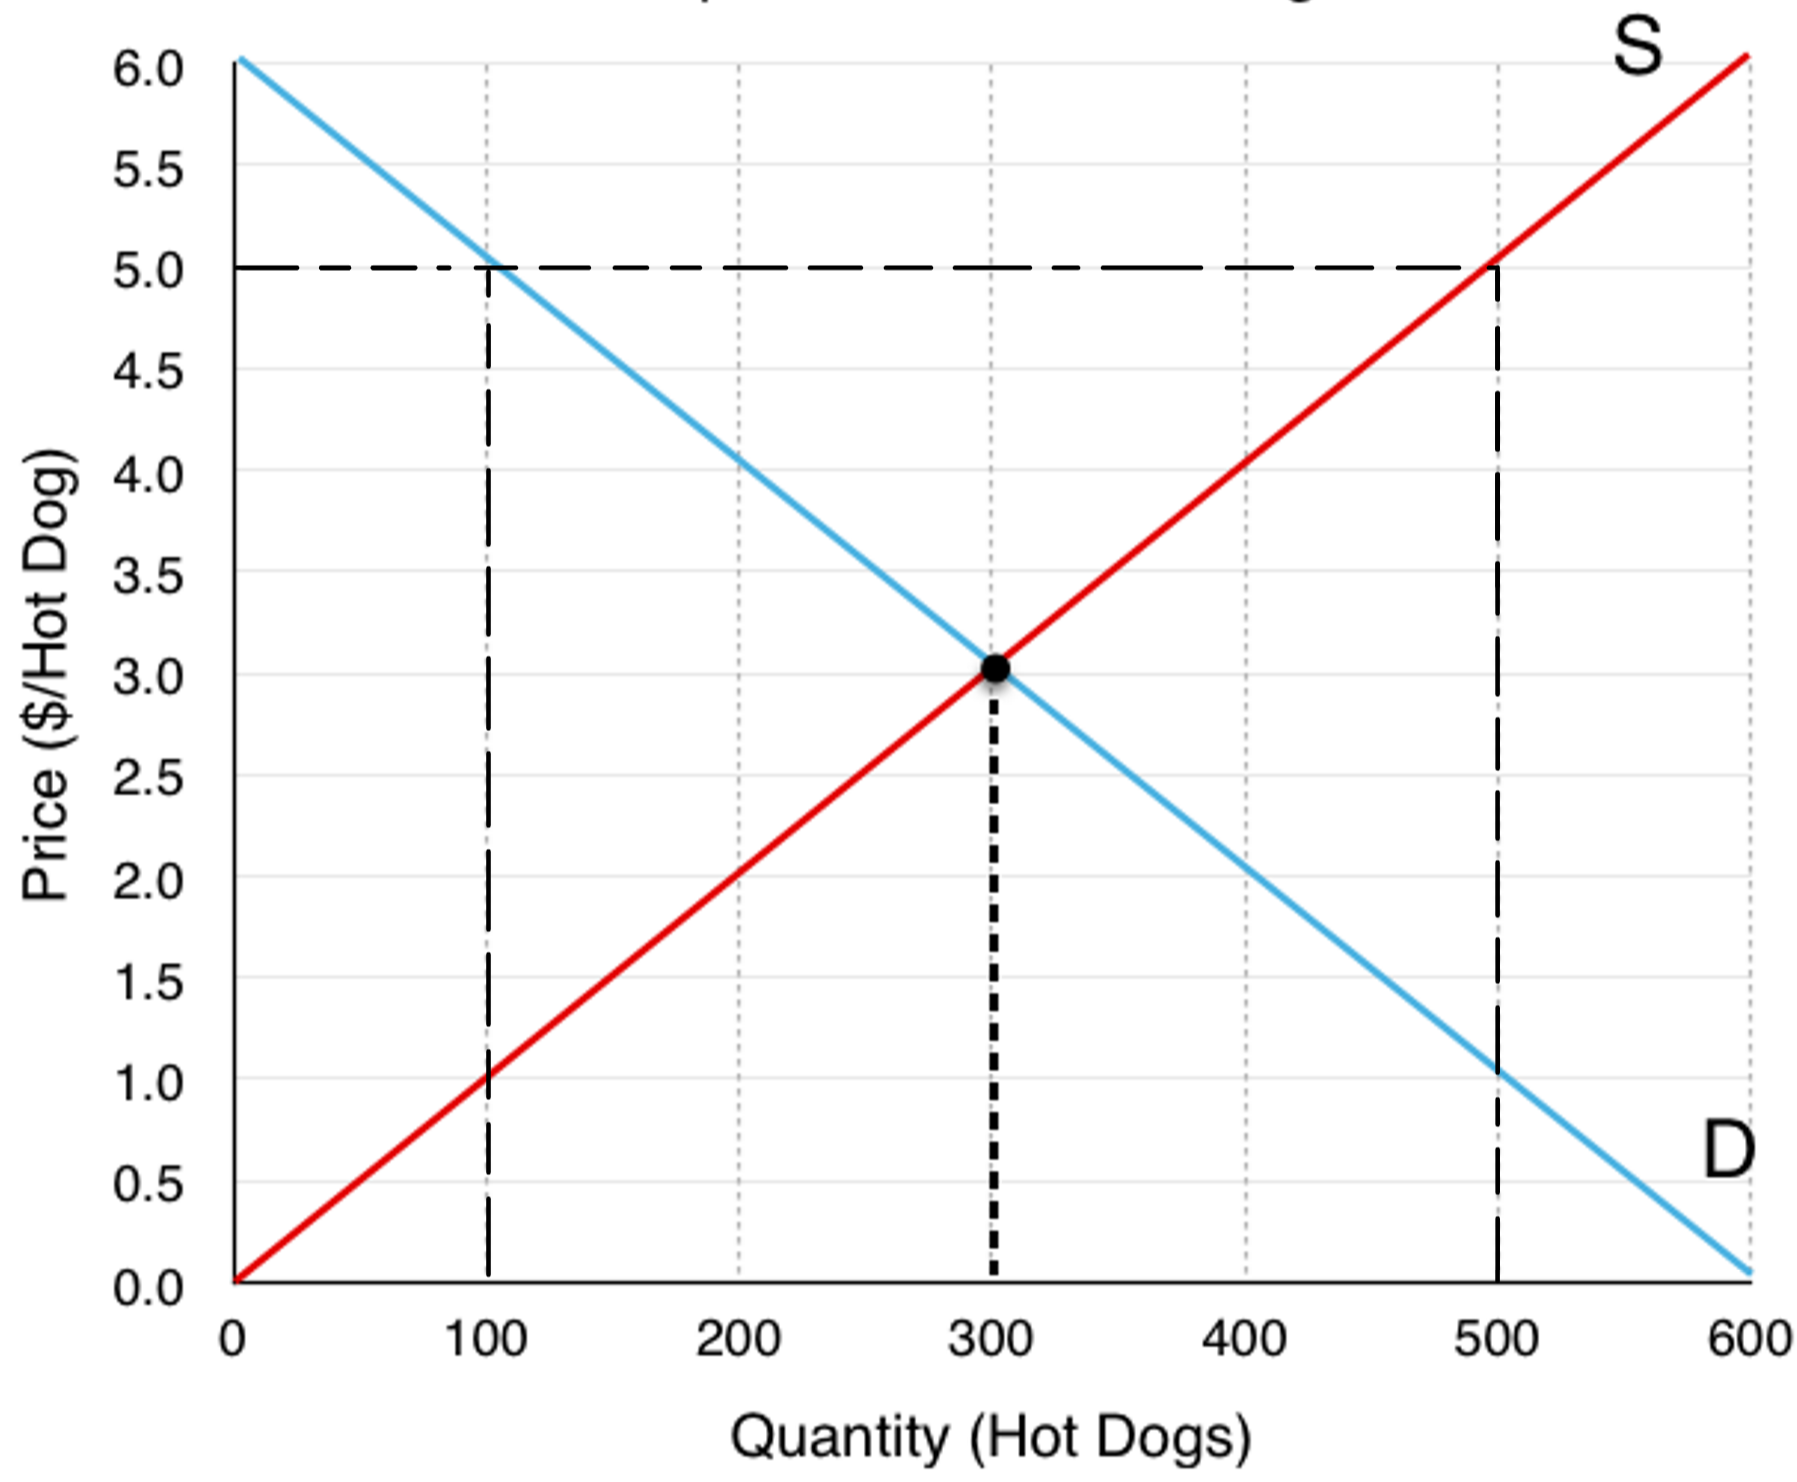
\includegraphics[width=5cm]{above market price.png}
        \end{figure}
        \item In this case, the quantity demanded was 100, while the quantity supplied was 500. What is this called?
        
        \item A \underline{surplus}, because the quantity supplied exceeded the quantity demanded
    \end{itemize}
\end{frame}

\begin{frame}{A Surplus}
    \begin{itemize}[<+->]
        \item When the price is above the equilibrium, such that there is a surplus, whose responsibility is it to raise the price?
        \begin{itemize}
            \item It's the \underline{producers'} responsibility to lower the price that they advertise to consumers
            \item Technically, both parties are responsible for agreeing upon a (lower) price, but the offer to lower the price is always implied by consumers, since they directly benefit from it
        \end{itemize}
        \item Once producers offer to sell for less, the price falls, the size of the surplus (in our example: 400) falls, and we repeat until equilibrium
    \end{itemize}
\end{frame}



\begin{frame}{Price Controls}
    \begin{itemize}[<+->]
        \item That is what happens in a free (unregulated) market
        \item What happens if we put regulations on the market?
        \item What sorts of regulations does the government use?
        \begin{enumerate}
            \item Taxes \& subsidies
            \item Quotas
            \item Price Floors and Price Ceilings
        \end{enumerate}
        \item Today, we will focus on price floors and ceilings, which are ``hard" price controls, in the sense that they place a fixed limit on the price of a good, 
        \begin{itemize}
            \item Taxes, on the other hand, are ``soft": they influence market price, without placing an absolute limit on what it can or cannot be
            \item Quotas are also a hard limit, but on quantity instead of price; we may not discuss quotas in great detail
        \end{itemize}

    \end{itemize}
\end{frame}


\begin{frame}{Definitions}
    \begin{itemize}[<+->]
        \item A \underline{\textbf{Price Ceiling}} is a legal maximum on the price at which a good can be sold
        \item A \underline{\textbf{Price Floor}} is a legal minimum on the price at which a good can be sold
        \item A \underline{\textbf{Shortage}} is a situation in which quantity demanded is greater than quantity supplied
        \item A \underline{\textbf{Surplus}} is a situation in which quantity supplied is greater than quantity demanded
    \end{itemize}
\end{frame}


\begin{frame}{Effective Price Ceiling/Floor}
    \begin{figure}
        \centering
        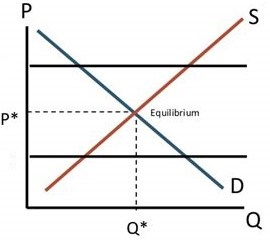
\includegraphics[width=6cm]{Inkednon-labelled controls.jpg}
        \caption*{Based on common sense, which of these should be called an effective price ceiling and effective price floor? \visible<2->{The top one is the ceiling, and the bottom the floor?}}
    \end{figure}
\end{frame}

\begin{frame}{}
    \begin{figure}
        \centering
        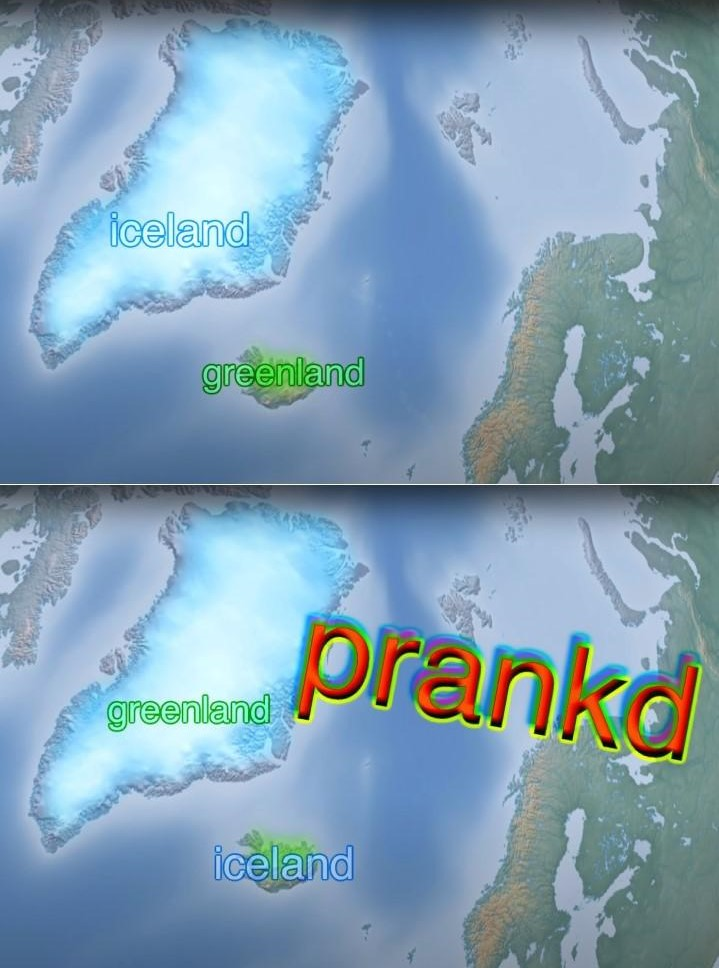
\includegraphics[height=7.5cm, width=10cm]{prankd.jpg}
        \vspace{-2mm}
        \caption*{Unfortunately, it's the other way around}
    \end{figure}
\end{frame}

\section*{Price Floors}

\begin{frame}{Price Floors}
    \begin{itemize}[<+->]
        \item A price floor is a legal minimum on the price at which a good can be sold
        \item Put another way, the price has to be above the price floor, it cannot be below
        \begin{itemize}
            \item This is why it is called a price floor: everything is above it, much like the floor in a room
        \end{itemize}
        \item Why implement a price floor? 
        \begin{itemize}
            \item If there is a minimum on the price of a good, that means that the government wants to assist suppliers: they want to guarantee that the supplier gets a minimum price for their work
            \item Examples: minimum wage, NFL tickets (until 2016), alcohol (Scotland)
            \item In practice, many governments, including our own, enforce keep what is essentially a price floor on many agricultural products (dairy, sugar, corn, etc.)  in place by buying up the excess of a product whenever it dips below a specific price, essentially stimulating demand, but then stopping when the price hits the floor
            \begin{itemize}
                \item While modelling this on a S/D graph looks a little different, it is \textit{de facto} a floor
            \end{itemize}
        \end{itemize}
    \end{itemize}
\end{frame}

\begin{frame}{An Ineffective Price Floor}
    \begin{itemize}[<+->]
        \item So what happens when a price floor is below the equilibrium price?
        \begin{figure}
            \centering
            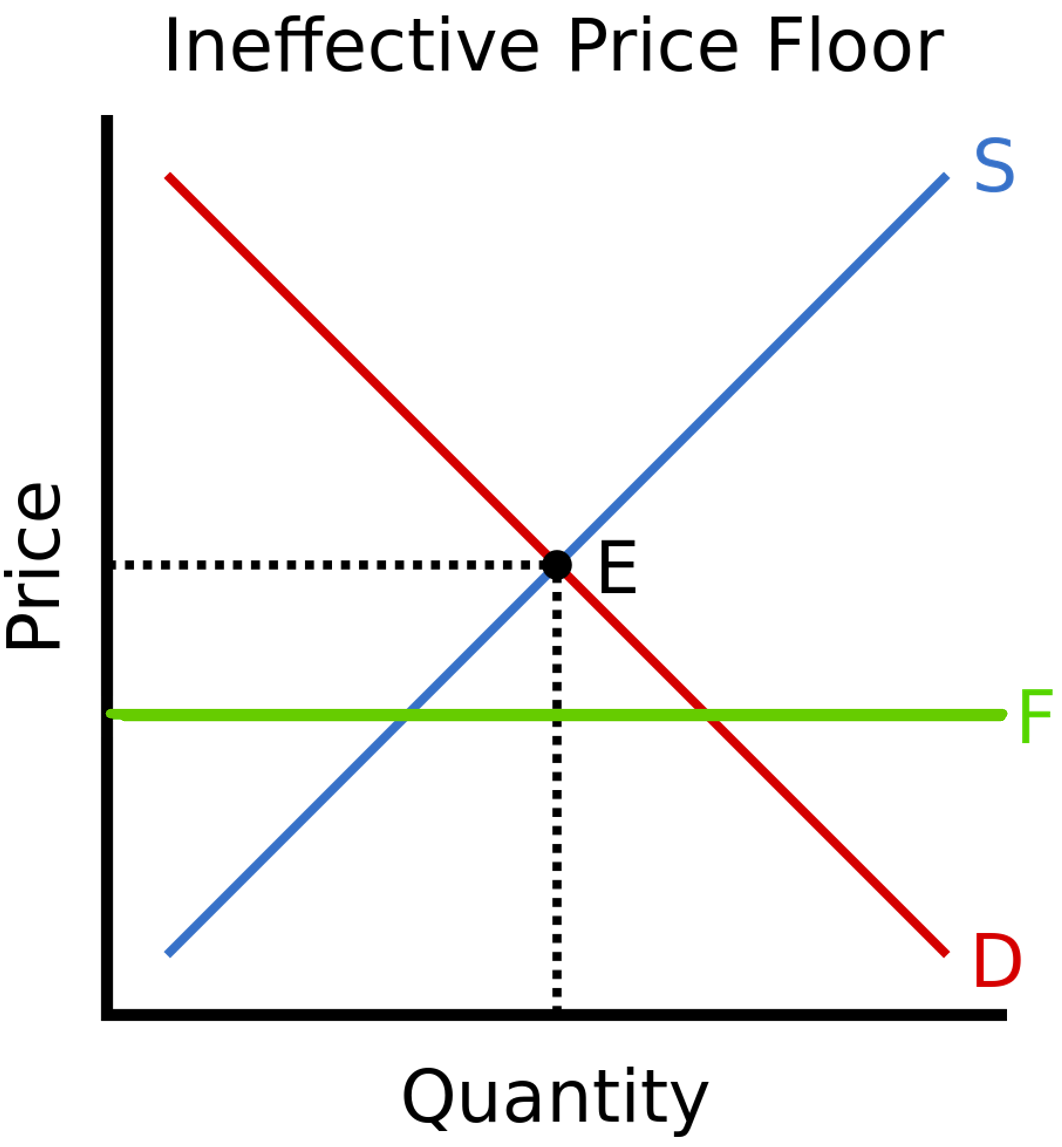
\includegraphics[width = 5cm]{Ineffective_Price_Floor.png}
            \caption*{To help you remember which is a floor vs. ceiling, you may want to include up arrows on your floor, to show that the price must be above it}
        \end{figure}
    \end{itemize}
\end{frame}

\begin{frame}{An Ineffective Price Floor (cont.)}
    \begin{itemize}[<+->]
        \item So what happens when a price floor is below the equilibrium price?
        \begin{figure}
            \centering
            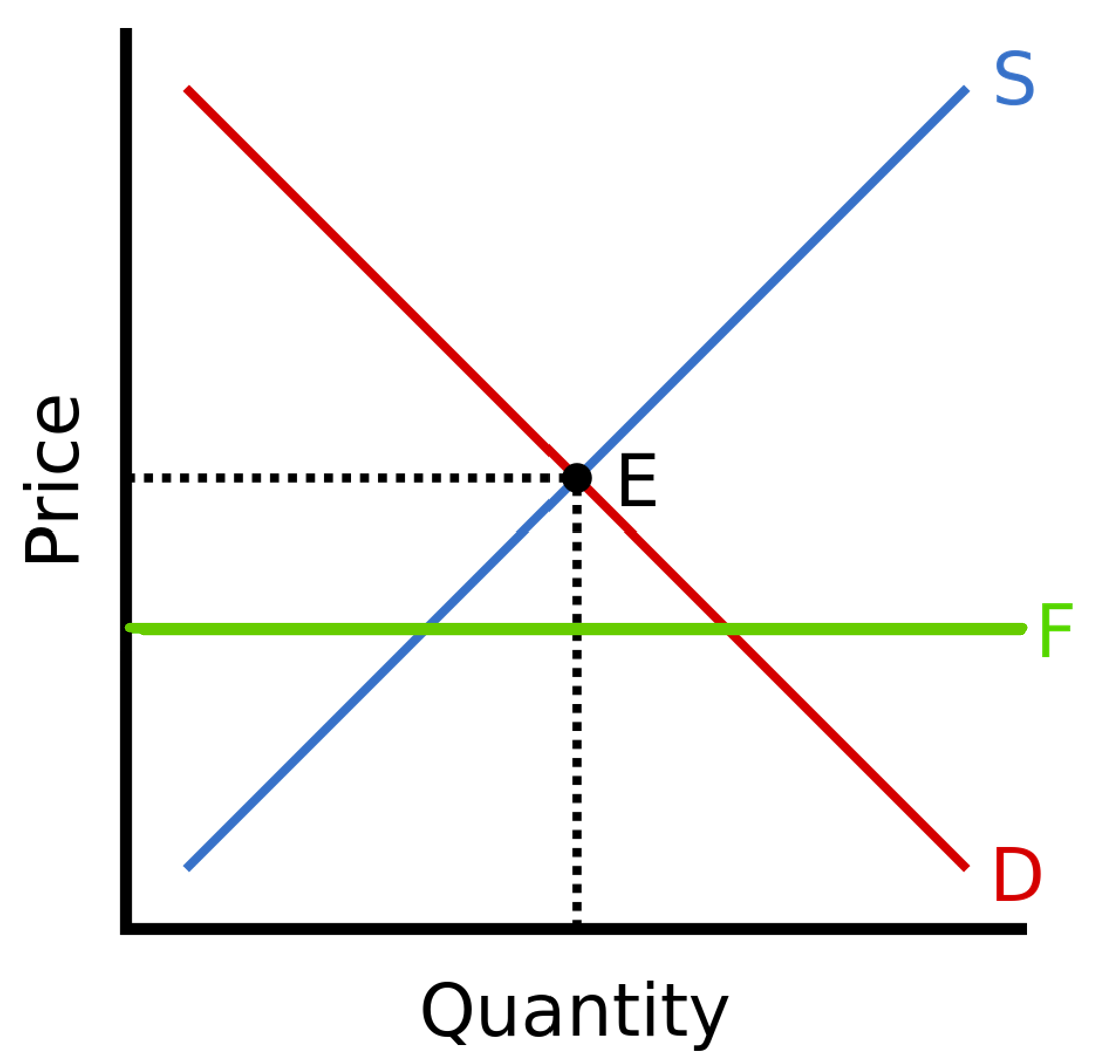
\includegraphics[width = 3cm]{Ineffective_Price_Floor unlab.png}
        \end{figure}
        \item In this case, the price is allowed to be above the floor, including at equilibrium
        \item So if the price started at the floor, consumers would increase their offers, and the price would rise to equilibrium (like we originally discussed)
        \item Thus, a price floor below the equilibrium price does nothing; it is useless
    \end{itemize}
\end{frame}


\begin{frame}{An Effective Price Floor}
    \begin{itemize}[<+->]
        \item So if setting the floor below is ineffective, what about setting one above the equilibrium?
        \begin{figure}
            \centering
            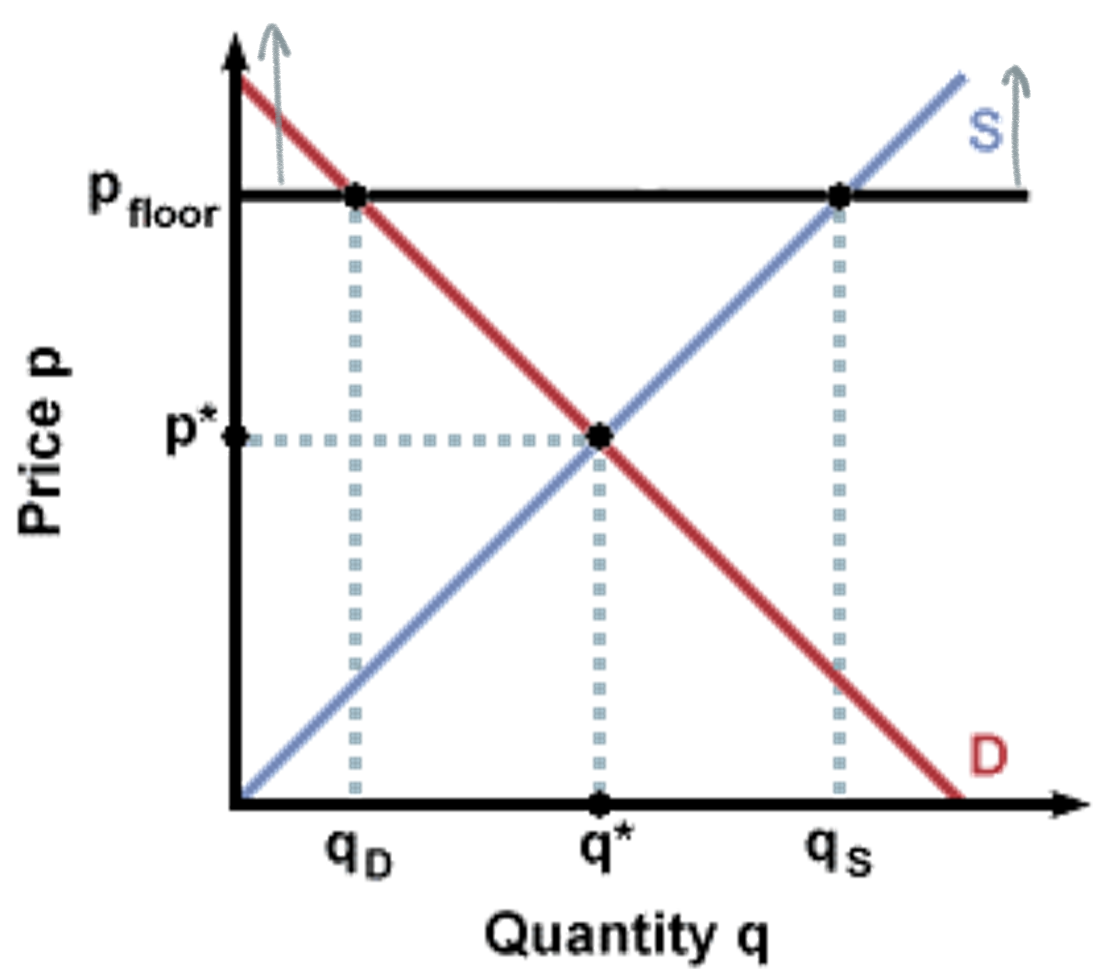
\includegraphics[width = 4cm]{effective price floor.png}
        \end{figure}
        \item Now, since the price is \underline{not} allowed below the floor, we cannot be at equilibrium
        \item However, the same market forces which drive us toward equilibrium will drive us to the price floor 
    \end{itemize}
\end{frame}


\begin{frame}{An Effective Price Floor (cont.)}
    \begin{itemize}[<+->]
        \item That is, if the price starts above the price floor, producers will make lower offers to attract consumers, until we are at the legal minimum 
        \item When the price is at the price floor, what effect does this have on the market?
        \item It will leave us with a surplus
        \begin{figure}
            \centering
            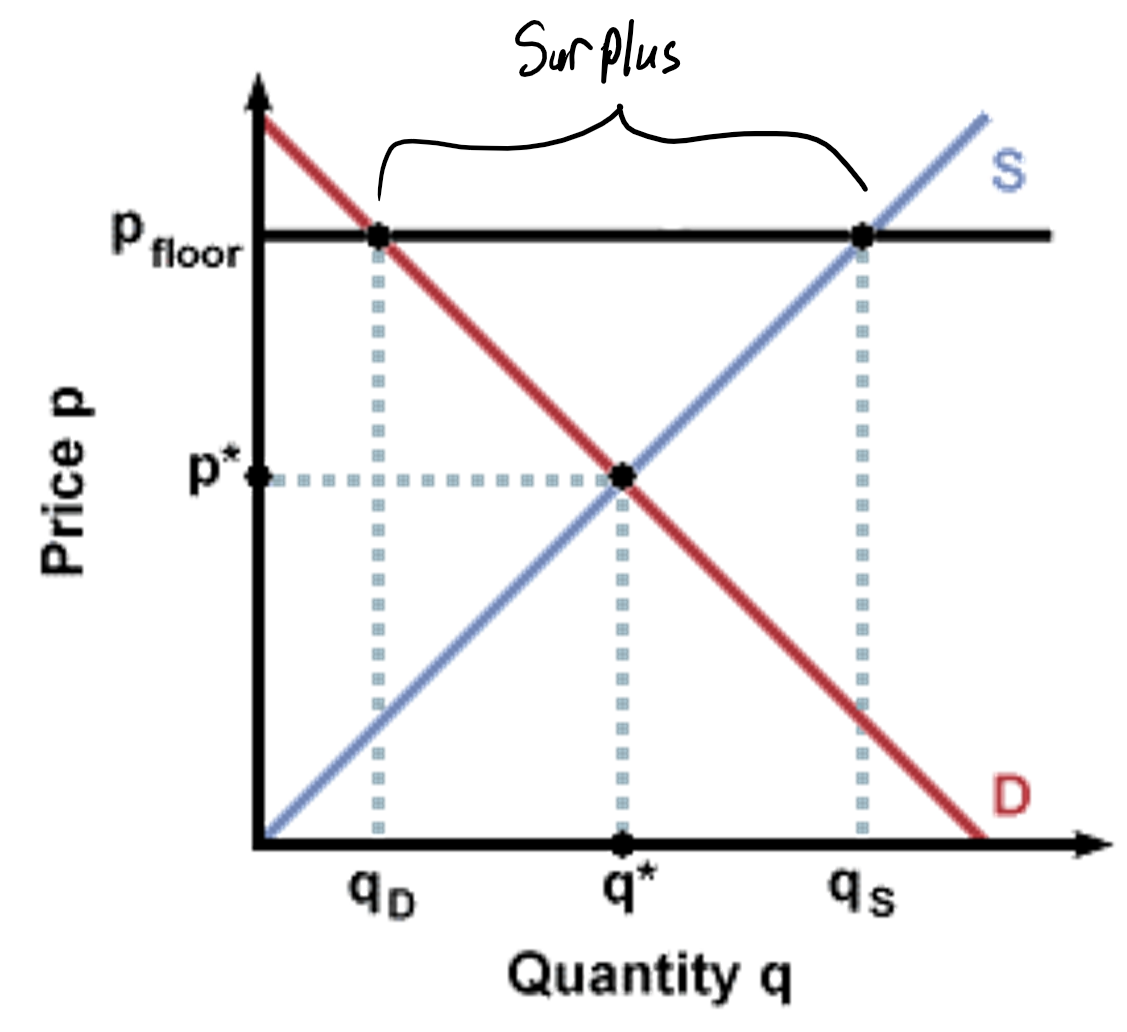
\includegraphics[width = 4cm]{price floor surplus.png}
        \end{figure}
        \item The size of the surplus will be $q_{s}-q_{d}$
    \end{itemize}
\end{frame}

%%%%%%%% Price Ceilings
\section*{Price Ceilings}

\begin{frame}{Price Ceilings}
    \begin{itemize}[<+->]
        \item A price ceiling is a legal maximum on the price at which a good can be sold
        \item Put another way, the price has to be below the price ceiling, it cannot be above
        \begin{itemize}
            \item This is why it is called a price ceiling: everything is below it, much like the ceiling in a room
        \end{itemize}
        \item Why implement a price ceiling? 
        \begin{itemize}
            \item If there is a maximum on the price of a good, that means that the government wants to assist consumers: they want to guarantee that the price doesn't get too out of hand for the consumer, or that it remains accessible to a greater population
            \item Examples: Rent caps in New York, wage caps in sports, insurance in Florida, possibly food
            \item Related: Other than an actual price ceiling, governments sometimes put a ceiling on how much a price can grow in terms of percent, such as rent in some states, or the price of housing in California 
        \end{itemize}
    \end{itemize}
\end{frame}

\begin{frame}{An Ineffective Price Ceiling}
    \begin{itemize}[<+->]
        \item So what happens when a price ceiling is above the equilibrium price?
        \begin{figure}
            \centering
            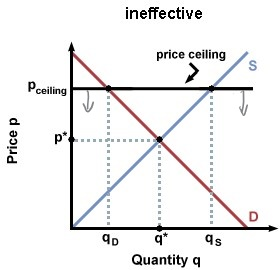
\includegraphics[width = 5cm]{Ineffective_Price_ceiling.jpg}
            \caption*{To help you remember which is a floor vs. ceiling, you may want to include \textit{down} arrows on your ceiling, to show that the price must be below it}
        \end{figure}
    \end{itemize}
\end{frame}

\begin{frame}{An Ineffective Price Ceiling (cont.)}
    \begin{itemize}[<+->]
        \item So what happens when a price ceiling is below the equilibrium price?
        \begin{figure}
            \centering
            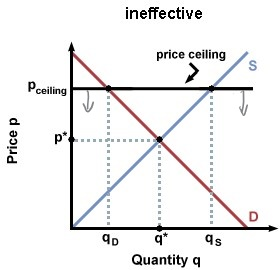
\includegraphics[width = 3cm]{Ineffective_Price_ceiling.jpg}
        \end{figure}
        \item In this case, the price is allowed to be below the ceiling, including at equilibrium
        \item So if the price started at the ceiling, producers would decrease their offers, and the price would fall to equilibrium (like we originally discussed)
        \item Thus, a price ceiling above the equilibrium price does nothing; it is useless
    \end{itemize}
\end{frame}


\begin{frame}{An Effective Price Ceiling}
    \begin{itemize}[<+->]
        \item So if setting the ceiling above is ineffective, what about setting one below the equilibrium?
        \begin{figure}
            \centering
            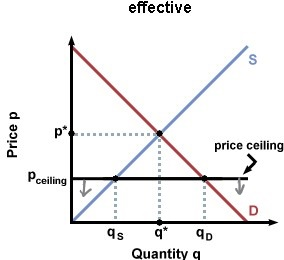
\includegraphics[width = 4cm]{Inkedeffective price ceiling.jpg}
        \end{figure}
        \item Now, since the price is \underline{not} allowed above the ceiling, we cannot be at equilibrium
        \item However, the same market forces which drive us toward equilibrium will drive us to the price ceiling 
    \end{itemize}
\end{frame}


\begin{frame}{An Effective Price Ceiling (cont.)}
    \begin{itemize}[<+->]
        \item That is, if the price starts below the price ceiling, consumers will make higher offers, until we are at the legally maximum price 
        \item When the price is at the price ceiling, what effect does this have on the market?
        \item It will leave us with a shortage
        \begin{figure}
            \centering
            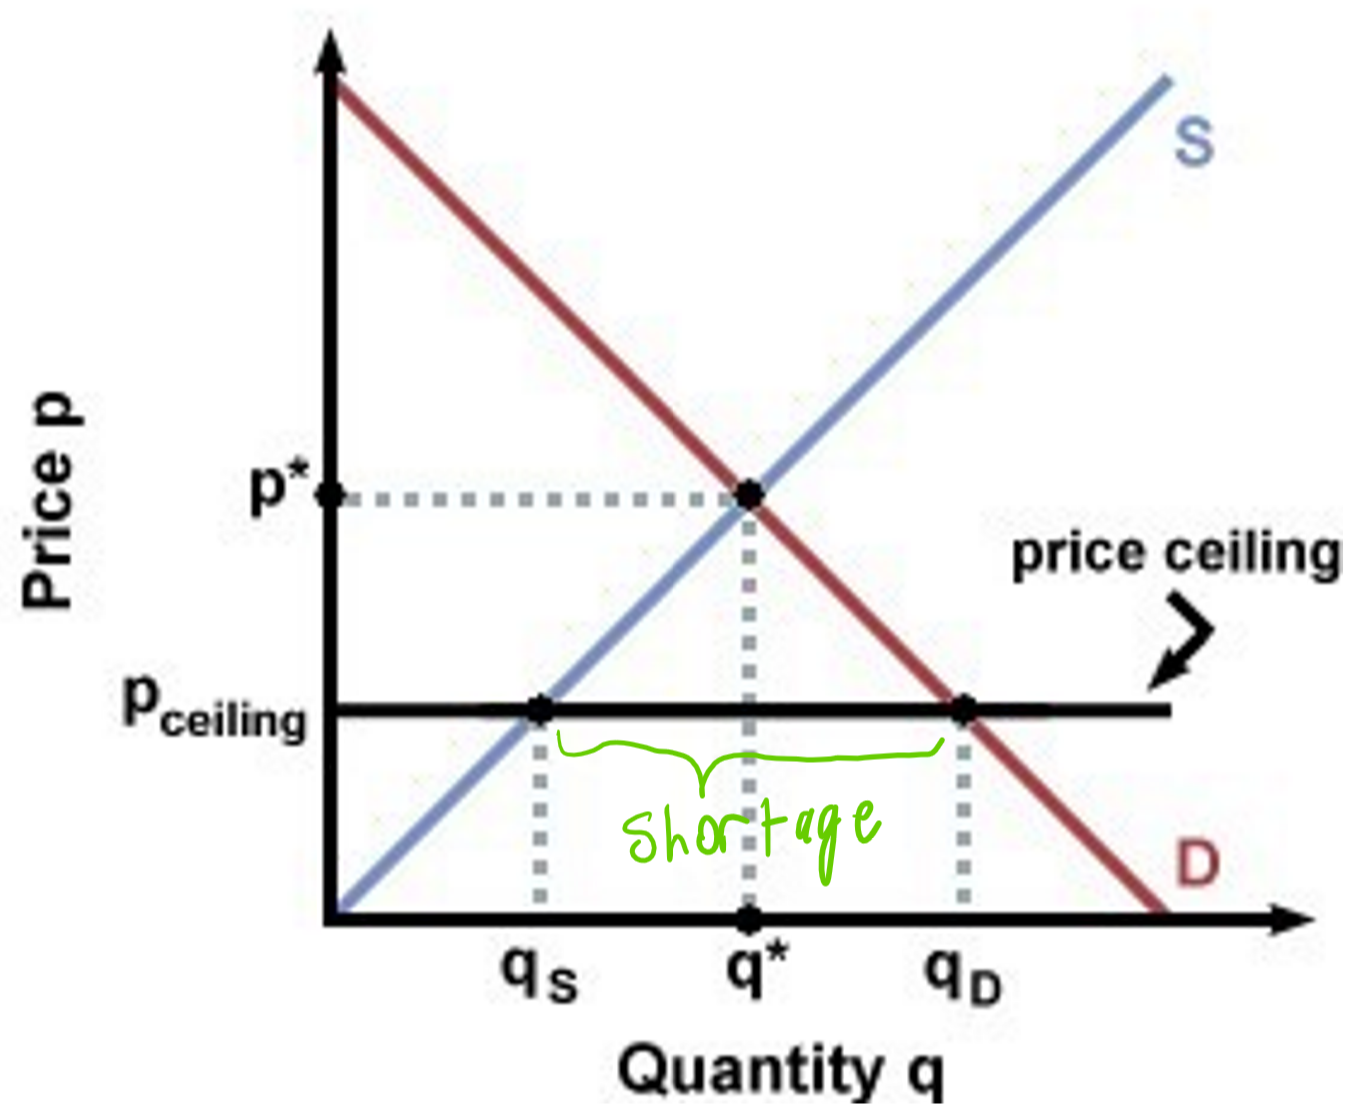
\includegraphics[width = 4cm]{price ceiling shortage.png}
        \end{figure}
        \item The size of the shortage will be $q_{d}-q_{s}$
    \end{itemize}
\end{frame}


\begin{frame}{Effective Price Controls}
    \begin{itemize}[<+->]
        \item An effective price ceiling goes \underline{below} an equilibrium
        \item An effective price floor goes \underline{above} an equilibrium
        \item In general, either of the lines shown in the aforementioned graph can be a price ceiling or floor, but if I also qualify that the price control is ``effective", you should be able to tell which is which
        \begin{itemize}
            \item An effective floor is above, an effective ceiling is below
        \end{itemize}
    \end{itemize}
\end{frame}


\begin{frame}{A Note about Ineffective Controls}
    \begin{itemize}[<+->]
        \item The government might still put into place an ineffective price control. Why?
        \item In the case of a floor, they may want to shield against a large drop in demand, or a huge technological innovation for supply
            \begin{figure}[H]
                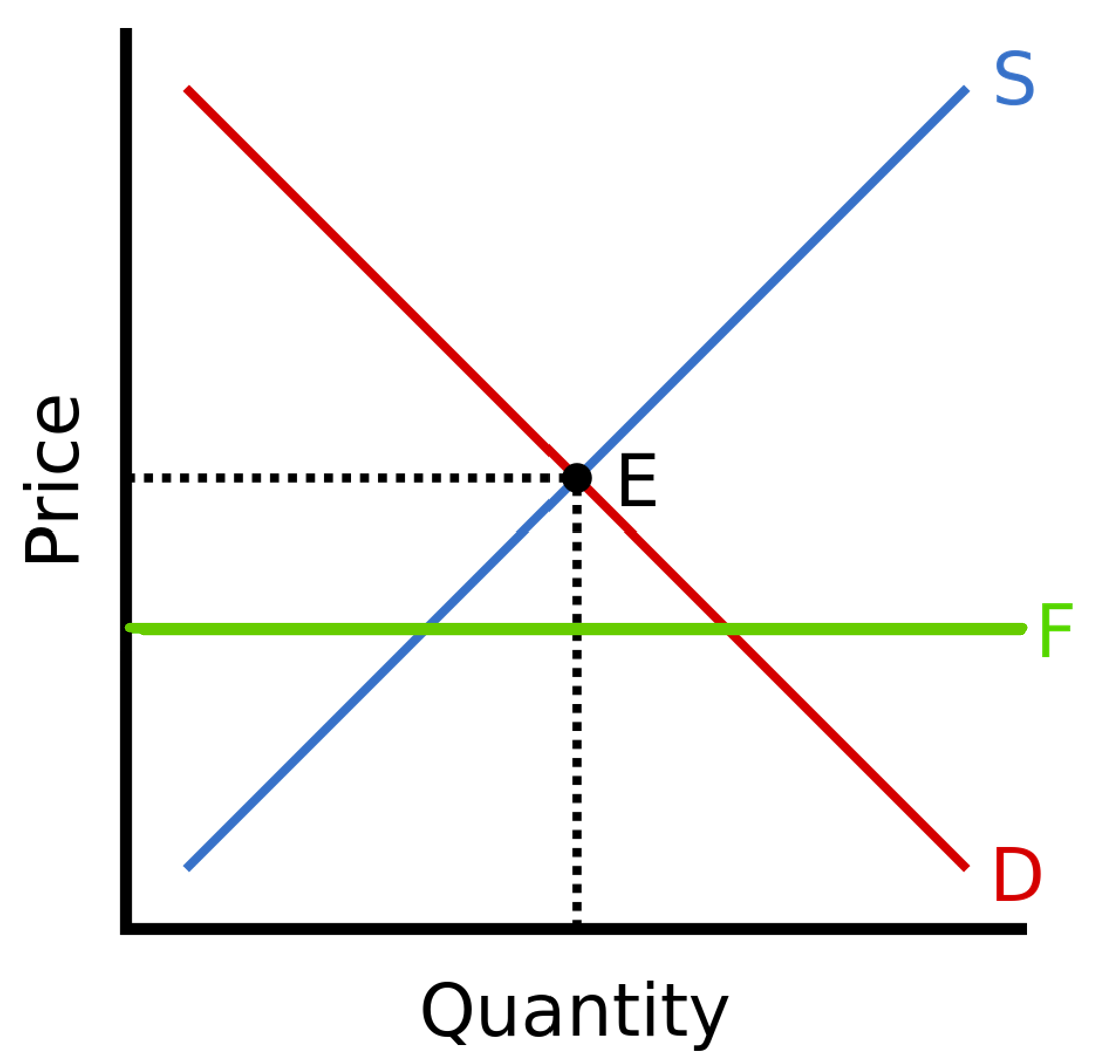
\includegraphics[width = 3cm]{Ineffective_Price_Floor unlab.png} 
            \end{figure} 
        \item In the above figure, a negative demand shock or positive supply shock would lead to the price dipping below the floor, which the government may not want
        \item The reverse justification would be valid for protecting consumers from negative supply or positive demand shocks
    \end{itemize}
\end{frame}









\end{document}